% Sablon pentru realizarea lucrarii de licenta, conform cu recomandarile
% din ghidul de redactare:
% - https://fmi.unibuc.ro/finalizare-studii/
% - https://drive.google.com/file/d/1xj9kZZgTkcKMJkMLRuoYRgLQ1O8CX0mv/view

% Multumiri lui Gabriel Majeri, acest sablon a fost creat pe baza
% codului sursa a lucrarii sale de licenta. 
% Codul sursa: https://github.com/GabrielMajeri/bachelors-thesis
% Website: https://www.gabrielmajeri.ro/
%
% Aceast sablon este licentiat sub Creative Commons Attribution 4.0 International License.

\documentclass[12pt, a4paper]{report}

% Suport pentru diacritice și alte simboluri
\usepackage{fontspec}

% Suport pentru mai multe limbi
\usepackage{polyglossia}

% Setează limba textului la română
\setdefaultlanguage{romanian}
% Am nevoie de engleză pentru rezumat
\setotherlanguages{english}

% Indentează și primul paragraf al fiecărei noi secțiuni
\SetLanguageKeys{romanian}{indentfirst=true}

% Suport pentru diferite stiluri de ghilimele
\usepackage{csquotes}

\DeclareQuoteStyle{romanian}
  {\quotedblbase}
  {\textquotedblright}
  {\guillemotleft}
  {\guillemotright}

% Utilizează biblatex pentru referințe bibliografice
\usepackage[
    maxbibnames=50,
    sorting=nty
]{biblatex}

\addbibresource{bibliography.bib}

% Setează spațiere inter-linie la 1.5
\usepackage{setspace}
\onehalfspacing

% Modificarea geometriei paginii
\usepackage{geometry}

% Include funcțiile de grafică
\usepackage{graphicx}
% Încarcă imaginile din directorul `images`
\graphicspath{{./images/}}

\usepackage{float}

% culori aditionale
\usepackage[dvipsnames]{xcolor}

% Listări de cod
\usepackage{listings}
\usepackage[newfloat]{minted}
\usepackage{caption}
% caption pentru listari de cod
\newenvironment{code}{\captionsetup{type=listing}}{}
\SetupFloatingEnvironment{listing}{name=Cod Sursă}

% Linkuri interactive în PDF
\usepackage[
    colorlinks,
    linkcolor={black},
    menucolor={black},
    citecolor={black},
    urlcolor={blue}
]{hyperref}

% Simboluri matematice codificate Unicode
\usepackage[warnings-off={mathtools-colon,mathtools-overbracket}]{unicode-math}

% Comenzi matematice
\usepackage{amsmath}
\usepackage{mathtools}

% Formule matematice
\newcommand{\bigO}[1]{\symcal{O}\left(#1\right)}
\DeclarePairedDelimiter\abs{\lvert}{\rvert}

% Suport pentru rezumat în două limbi
% Bazat pe https://tex.stackexchange.com/a/70818
\newenvironment{abstractpage}
  {\cleardoublepage\vspace*{\fill}\thispagestyle{empty}}
  {\vfill\cleardoublepage}
\renewenvironment{abstract}[1]
  {\bigskip\selectlanguage{#1}%
   \begin{center}\bfseries\abstractname\end{center}}
  {\par\bigskip}

% Suport pentru anexe
\usepackage{appendix}

% Stiluri diferite de headere și footere
\usepackage{fancyhdr}

% Metadate
\title{Dezvoltarea unei aplicații educaționale bazată pe flashcard-uri: Alfie}
\author{Radu George-Mihai}

% Generează variabilele cu @
\makeatletter

\begin{document}

% Front matter
\cleardoublepage
\let\ps@plain

% Pagina de titlu
\begin{titlepage}

% Redu marginile
\newgeometry{left=2cm,right=2cm,bottom=1cm}

\begin{figure}[!htb]
    \centering
    \begin{minipage}{0.2\textwidth}
        
\includegraphics[width=\linewidth]{logo-ub.png}
    \end{minipage}
    \begin{minipage}{0.5\textwidth}
        \large
        \vspace{0.2cm}
        \begin{center}
            \textbf{UNIVERSITATEA DIN BUCUREȘTI}
        \end{center}
        \vspace{0.3cm}
        \begin{center}
            \textbf{
                FACULTATEA DE \\
                MATEMATICĂ ȘI INFORMATICĂ
            }
        \end{center}
    \end{minipage}
    \begin{minipage}{0.2\textwidth}
        
\includegraphics[width=\linewidth]{logo-fmi.png}
    \end{minipage}
\end{figure}

\begin{center}
\textbf{SPECIALIZAREA INFORMATICĂ}
\end{center}

\vspace{1cm}

\begin{center}
\Large \textbf{Lucrare de licență}
\end{center}

\begin{center}
\huge \textbf{\MakeUppercase{\@title}}
\end{center}

\vspace{3cm}

\begin{center}
\large \textbf{Absolvent \\ \@author}
\end{center}

\vspace{0.25cm}

\begin{center}
\large \textbf{Coordonator științific \\ Lect. dr. Radu-Ștefan Mincu}
\end{center}

\vspace{2cm}

\begin{center}
\Large \textbf{București, iunie-iulie 2023}
\end{center}
\end{titlepage}
\restoregeometry
\newgeometry{
    margin=2.5cm
}

\fancypagestyle{main}{
  \fancyhf{}
  \renewcommand\headrulewidth{0pt}
  \fancyhead[C]{}
  \fancyfoot[C]{\thepage}
}

\addtocounter{page}{1}

% Rezumatul
\begin{abstractpage}

\begin{abstract}{romanian}

Progresul tehnologic și inovațiile din sfera digitală au favorizat creșterea numărului de persoane care au acces la învățământ și studii superioare. Acesta reprezintă unul dintre motivele pentru care sunt create și dezvoltate diverse instrumente și platforme care să vină în sprijinul studenților, ba chiar și adulților.

Aplicația \textit{Alfie}, prezentată în cadrul acestei lucrări, își propune să ofere un suport educațional utilizatorilor săi (studenți) în timpul studiului. Aplicația este creată în variantă de mobil. Aplicația este de tip flashcard digital, cu suport pentru diverse formate de text. De asemenea, aplicația oferă suport și pentru inserarea și editarea de imagini în cartonașe, asigurând un suport vizual în procesul de învățare.

O caracteristică prin care se remarcă aplicația este reprezentată de suportul de obținere a textelor matematice din imagini în format tex, folosind un microserviciu, pentru o vizualizare mai bună și mai eficientă, în defavoarea pozelor cu rezoluție scăzută sau a textelor ilizibile. Alte funcționalități semnificative ale aplicației sunt: backup local și în cloud a cartonașelor și al conținutului media, statistici de învățare a cartonașelor, UI/UX ușor de folosit și customizabil.

\end{abstract}

\begin{abstract}{english}

\end{abstract}

Technological progress and innovations in the digital sphere have helped increase the number of people with access to education and higher education. This is one of the reasons why various tools and platforms are being created and developed to support students and even adults.

The application \textit{Alfie}, presented in this paper, aims to provide educational support to its users (students) during their studies. The app is created in a mobile version. The app is a digital flashcard type app with support for various text formats. The app also provides support for inserting and editing images in flashcards, providing visual support in the learning process.

A stand out feature of the application is the support for obtaining mathematical texts from tex images using a microservice for better and more efficient visualisation, at the expense of low resolution pictures or illegible text. Other significant features of the app are: local and cloud backup of cards and media content, card learning statistics, easy to use and customizable UI/UX.

\end{abstractpage}


\tableofcontents

% Main matter
\cleardoublepage
\pagestyle{main}
\let\ps@plain\ps@main

\chapter{Introducere}

\section{Context}

Este dovedit faptul că \textit{educația avansată} reprezintă motorul principal al progresului ce stă la baza obiectivelor de dezvoltare durabilă la nivel global. \textit{Educația terțiară} este percepută ca fiind catalistul pentru dezvoltare și sustenabilitate \cite{educationParticipantsOECD}. Așadar, se poate aprecia faptul că este imperios pentru societate să formeze cât mai multe persoane cu studii superioare absolvite în vederea atingerii dezvoltării și prosperității viitoarelor generații.

\begin{figure}[H]
    \centering
    \textbf{Tendințe în ponderile tinerilor cu vârste cuprinse între 25-34 de ani cu studii superioare (în perioada 2000 – 2021)}\par\medskip
    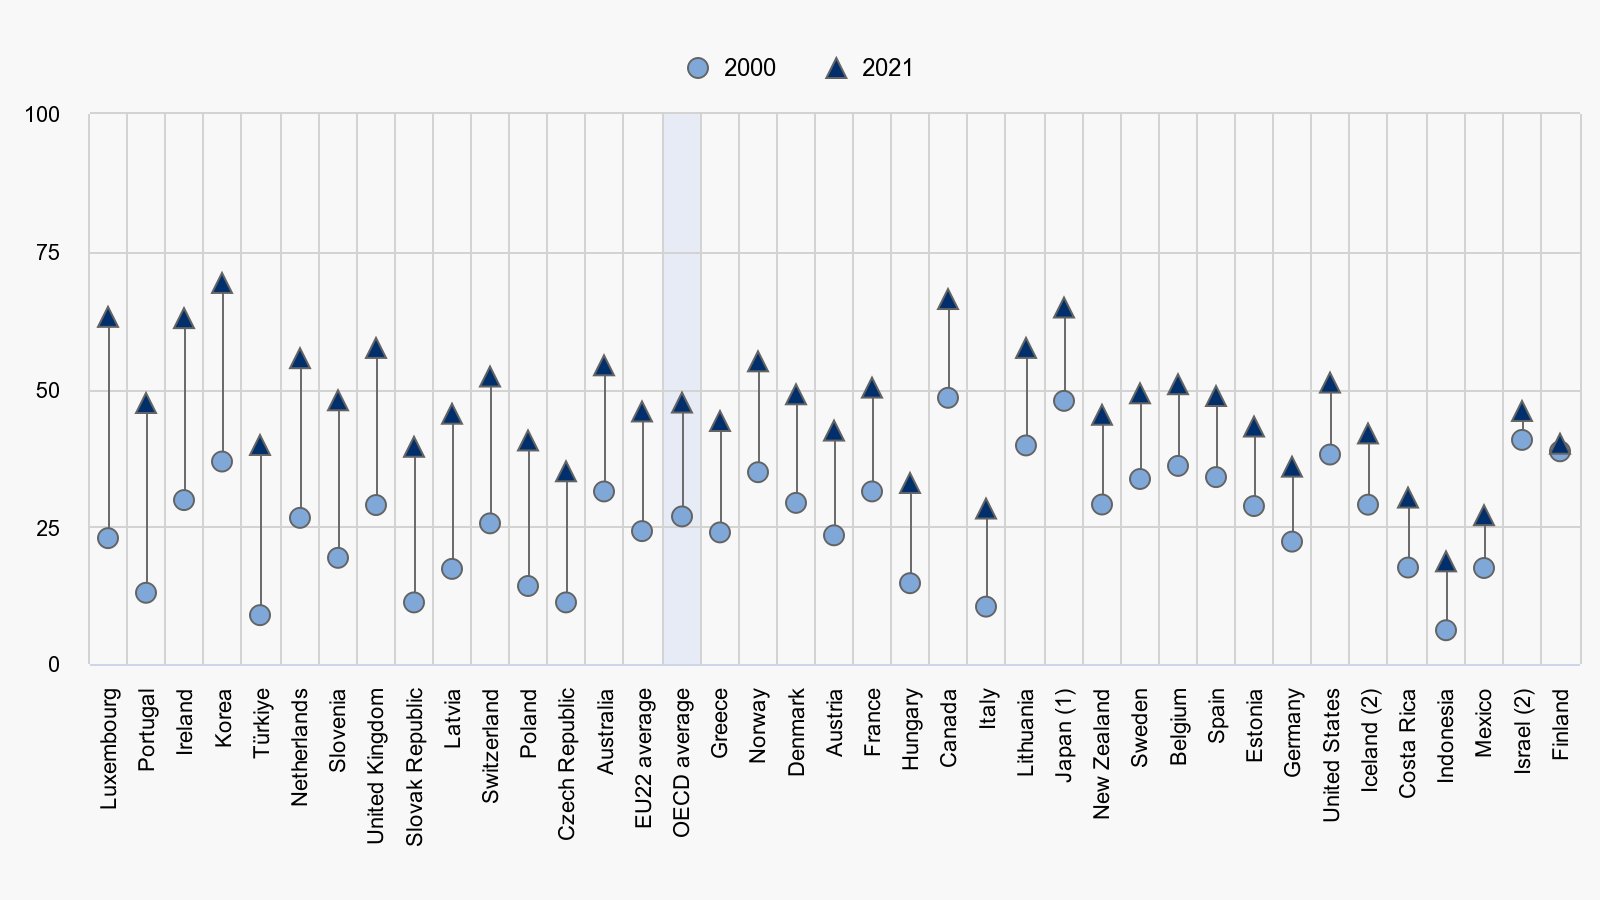
\includegraphics[width=.9\linewidth]{trends-tertiary-educated-adults.png}
    \caption{Țările sunt ordonate în funție de diferența procentuală de persoane cu studii superioare între anii 2000-2021. Datele includ și programele superioare după licență și cele post-secundare non-terțiare \cite{levelAdultsStudiedOECD}}
\end{figure}

Datorită condițiilor globale de natură economico-politică, înscrierile la școli au crescut, favorizate și de obligativitatea școlară la nivel de bază. Numărul persoanelor cu vârste cuprinse între 25 și 34 de ani ce au decis să urmeze un program de studii superioare s-a mărit foarte mult în majoritatea țărilor din OECD. Ponderea medie a tinerilor adulți care au studii superioare aproape s-a dublat în perioada 2000-2021 (de la aproximativ 27\% în 2000 la 48\% în 2021). Dacă trendul curent al educației digitalizate continuă să se dezvolte, se consideră că educația superioară va fi cea mai comună realizare printre adulții din spațiul muncii în următorii ani \cite{levelAdultsStudiedOECD}.

Pentru a încuraja și a ajuta tinerii în atingerea țelului de a obține o educație superioară, societatea a creat diferite materiale și produse care să vină în sprijinul studenților și a le facilita procesul de învățare continuă (de la cărți la materiale video, și diverse aplicații).

Printre numeroasele metode pe care le folosesc studenții și elevii în vederea eficientizării procesului de învățare se numără \textit{flashcard-urile}. Această metodă de învățare este populară atât în rândul studenților care trebuie să memoreze cât mai multe informații (precum cei de la medicină sau drept), cât și al elevilor care învață o nouă limbă străină. Studenții de la medicină sunt nevoiți să învețe un volum foarte mare de informații într-un timp cât mai scurt, motiv pentru care se folosesc de flashcard-uri pentru a fi cât mai eficienți posibil și a stoca informațiile în memoria de lungă durată \cite{in2med}.

Flashcard-urile pot varia de la a fi \textit{foarte simple} (caz în care cele mai importante cuvinte sunt colorate diferit) la a fi \textit{foarte complexe} (unde pot conține poze sau desene). S-a observat faptul că utilizarea culorilor cu scopul de a coda, a memora și a reîmprospăta informația reținută în memorie permite o creștere semnificativă a ratei de învățare, în special în rândul adulților \cite{journalEducation}.

\noindent\begin{minipage}{0.6\textwidth}
    \begin{figure}[H]
    \centering
    \textbf{Exemple de cartonașe pentru medicină}\par\medskip
    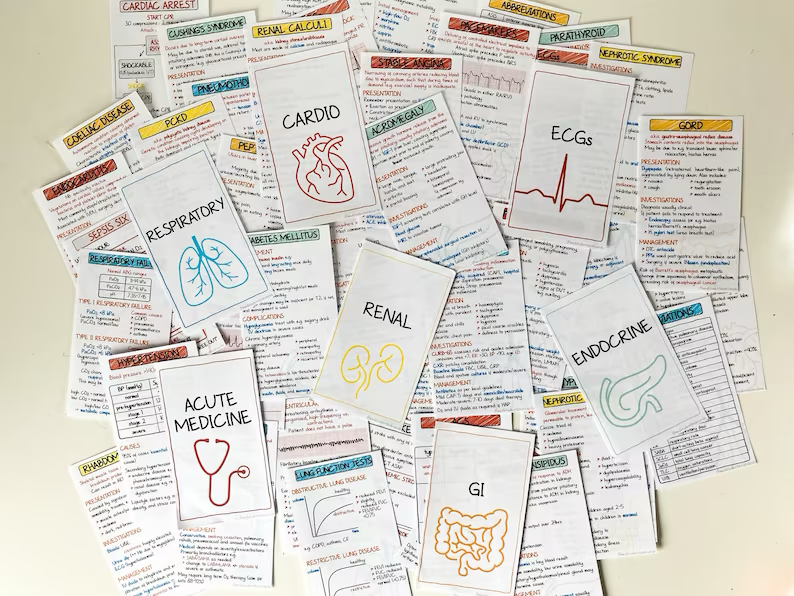
\includegraphics[width=\linewidth]{cartoanse-medicina-etsy.png}
    \caption{Diverse exemple de cartonașe pentru domeniul medicinii, folosindu-se de diferite desene, grafice și culori \cite{etsyPaperFlashCardsMedicine}} 
    \label{fig:cartonase}
    \end{figure}
\end{minipage}
\hfill
\begin{minipage}{0.35\textwidth}
    Înainte de era digitalizării, studenții foloseau flashcard-uri din hârtie (câteva exemple pot fi vizualizate în figura \ref{fig:cartonase}). Acestea prezintă, de asemenea, dezavantaje, întrucât pot fi dificil de prezervat și de gestionat.

    În prezent, există diverse aplicații educative de tip flashcard ce oferă multiple beneficii și un management eficient al acestora. În cele ce urmează sunt prezentate patru astfel de aplicații.
\end{minipage}

\subsection{Aplicații similare}

\subsubsection{Ankie}

\noindent\begin{minipage}{0.6\textwidth}
    Proiectul \textit{Ankie} \cite{anki} este unul din cele mai populare și mai complexe aplicații de tip flashcard similare. Anki oferă suport pentru imagini, audio, video și text științific pentru flashcard-uri. Printre principalele caracteristici se pot enumera: sincronizarea între dispozitive, aplicații pentru cele trei sisteme de operare pe desktop și laptop (Windows, Mac, Linux), dar și pentru mobil (Android și iOS). Proiectul este complet open source și are ca main selling feature faptul că este customizabil prin crearea de plugin-uri. Singura problemă menționată de utilizatori este aceea că aplicația este foarte complexă, ceea ce produce dificultăți persoanelor noi care tocmai au accesat aplicația.
\end{minipage} 
\hfill
\begin{minipage}{0.35\textwidth}
    \begin{figure}[H]
    \centering
    \textbf{Aplicația Ankie}\par\medskip
    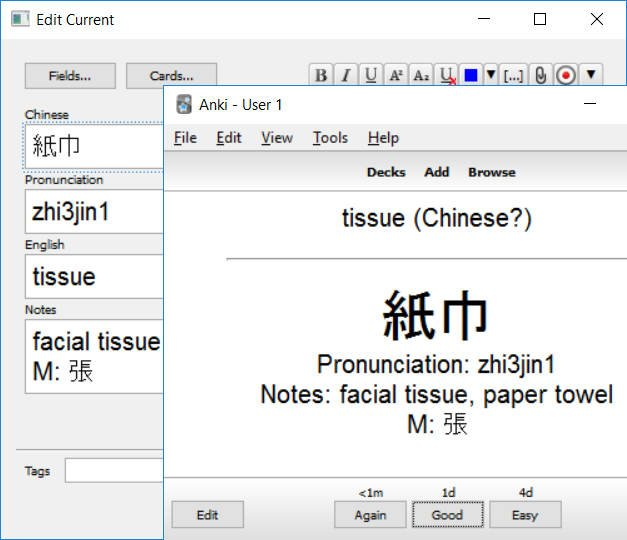
\includegraphics[width=\linewidth]{ankie.jpg}
    \caption{Exemplu de creare a unui cartonaș pentru o limbă străină \cite{ankiImageExample}} 
    \label{fig:exemplu_ankie}
    \end{figure}
\end{minipage}

\bigbreak
Caracterul de complexitate prezintă avantajul de a folosi proiectul Ankie în mai multe scopuri, precum învățarea unei noi limbi străine ori pregătirea pentru examene de medicină sau de drept. Alt avantaj ar fi faptul că nu este nevoie de un cont pentru a putea utiliza principalele caracteristici ale aplicației (excepție făcând sincronizarea cartonașelor între dispozitive).

\subsubsection{Memrise}

\noindent\begin{minipage}{0.35\textwidth}
    \begin{figure}[H]
        \centering
        \textbf{Aplicația Memrise}\par\medskip
        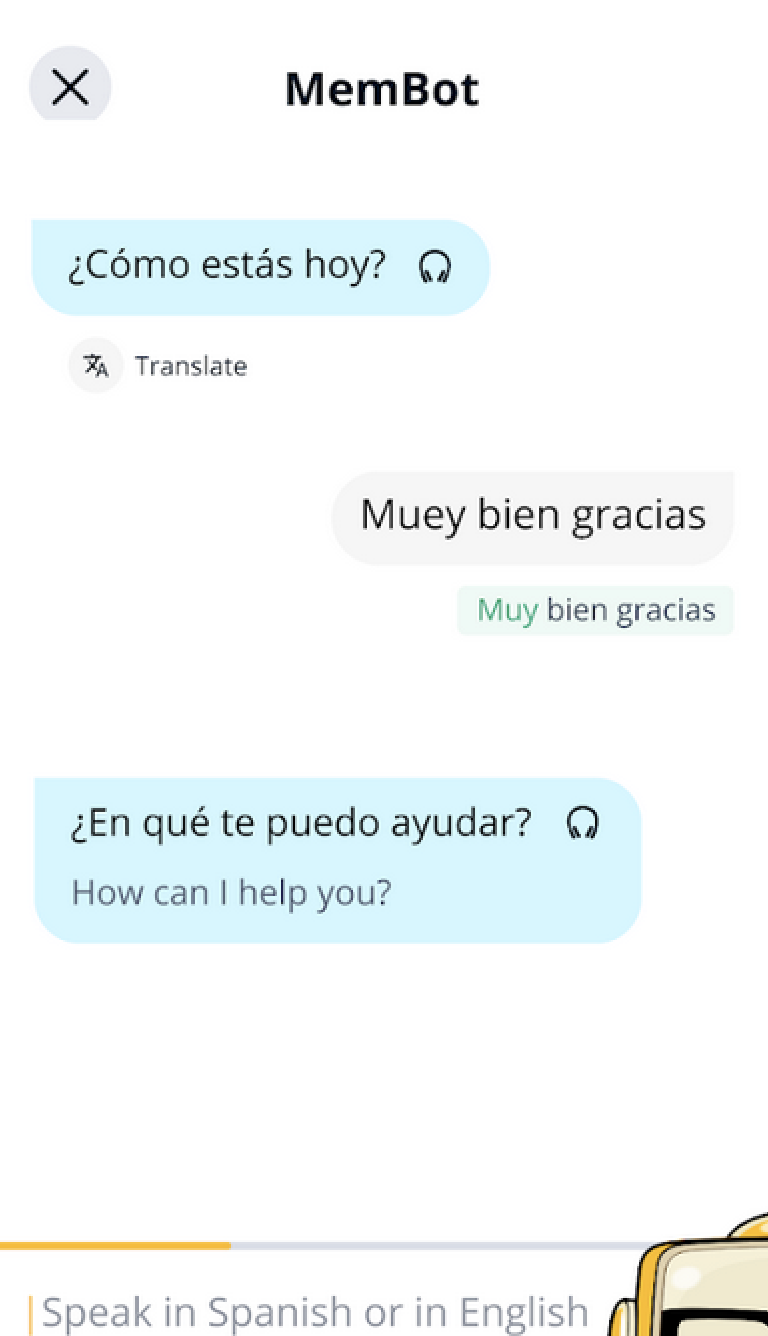
\includegraphics[width=.8\linewidth]{memrise.png}
        \caption{Exemplu de conversație în aplicația Memrise \cite{memriseImageExample}} 
        \label{fig:exemplu_memrise}
    \end{figure}
\end{minipage} 
\hfill
\begin{minipage}{0.55\textwidth}
   Aplicatia \textit{Memrise} \cite{memrise} este disponbilă doar pentru dispozitivele mobile. Principalul selling factor este de a învăța o nouă limbă străină. Proiectul oferă cursuri pentru 23 de limbi, ofera quizuri, videoclipuri cu traduceri de către vorbitori nativi. Un nou feature adus de această aplicație este practicarea vorbitului unei noi limbi folosind GPT-3, drept partener AI de conversație (exemplu în figura \ref{fig:exemplu_memrise}. Aplicația oferă atât un plan free cât și unul plătit și este de tip proprietar. Dezavantajul aplicației constă în faptul ca targetează doar învățarea limbilor străine, deși excelează în acest domeniu oferind cursuri.
\end{minipage}

\subsubsection{Quizlet}

\noindent\begin{minipage}{0.55\textwidth}
    Aplicatia \textit{Quizlet} \cite{quizlet} reprezintă un alt competitor, bazându-se pe acoperirea mai multor domenii, printre care se numără: examene, arte, limbi străine și științe. De asemenea, aceasta are un market pentru folosirea altor seturi de cartonașe pentru învățare. Anumite seturi de cartonașe „curated”, aparținând creatorilor aplicației, denotă unul dintre avantajele aplicației. Quizlet oferă atât un plan gratuit, cât și unul plătit, fiind de tip proprietar, ca în cazul aplicației Memrise. Dezavantajul aplicației Quizlet este reprezentat de faptul că planul gratuit are forma unui demo, ba mai mult, este destul de limitat în atragerea utilizatorilor. Un alt dezavantaj este acela că, fiind o aplicație proprietară, nu pot fi adăugate plugin-uri sau extensii.
\end{minipage} 
\hfill
\begin{minipage}{0.35\textwidth}
    \begin{figure}[H]
        \centering
        \textbf{Aplicația Quizlet}\par\medskip
        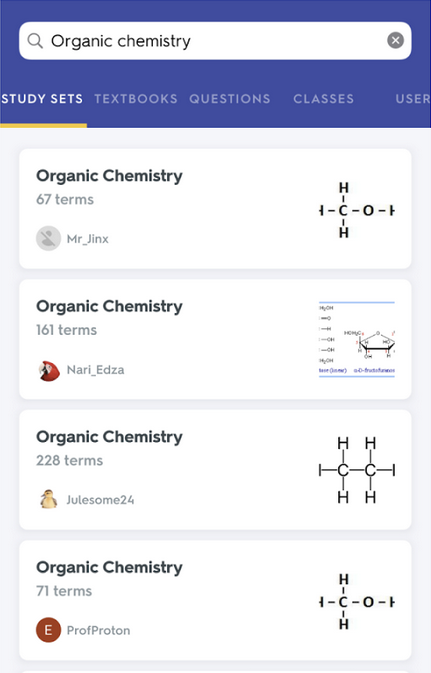
\includegraphics[width=\linewidth]{quizlet.png}
        \caption{Exemplu de pachete în aplicația Quizlet \cite{quizletImageExample}} 
        \label{fig:exemplu_quizlet}
    \end{figure}
\end{minipage}

\subsubsection{Brainscape}

\noindent\begin{minipage}{0.35\textwidth}
    \begin{figure}[H]
        \centering
        \textbf{Aplicația Brainscape}\par\medskip
        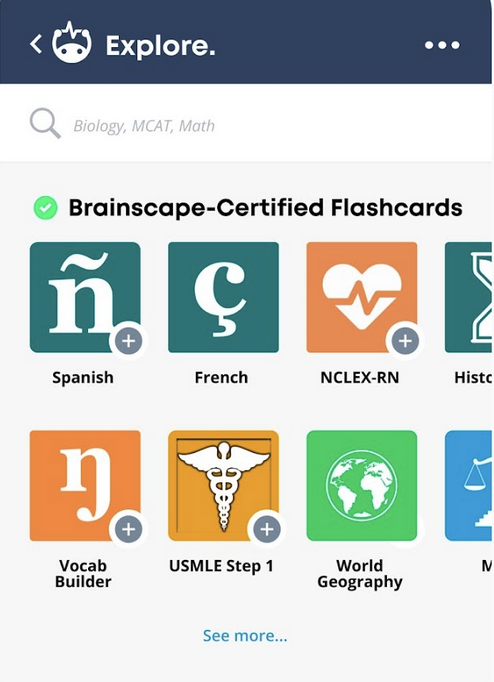
\includegraphics[width=\linewidth]{brainscape.png}
        \caption{Exemplu de pachete în aplicația Brainscape \cite{brainscapeImageExample}} 
        \label{fig:exemplu_brainscape}
    \end{figure}
\end{minipage} 
\hfill
\begin{minipage}{0.55\textwidth}
    Aplicația \textit{Brainscape} \cite{brainscape} reprezintă un alt competitor solid din acest segment. Principalii clienți ai aplicației activează în domeniul de business pentru training. Aceasta oferă suport pentru web și dispozitivele mobile, dar și planuri gratuite și plătite. Un avantaj ar consta în punerea la dispoziția utilizatorilor a unei game largi de cartonașe din varii domenii. Printre dezavantajele aplicației se numără suportul existent doar în versiunea de web, respectiv o aplicație proprietară fără suport pentru extensii.
\end{minipage}

\section{Scopul lucrării}

Scopul lucrării este acela de a crea o aplicație de mobil pentru principalele sisteme de operare (Android și iOS), orientată către studenții din STEM, care să le ofere un suport complementar în sistemul de învătare.

Aplicațiile prezentate în secțiunea anterioară au un public restrâns de utilizatori, motiv pentru care se urmărește ca noua aplicație creată să acopere o arie mai largă de nevoi. Astfel, aplicația \textit{Alfie} încurajează și crearea unor cartonașe de învățare pentru științele exacte, utilizările fiind, în principal, pentru ecuații și teoreme. Aplicația vine în ajutorul scrierii de text științific în cartonașe cu feature-ul de convertire a unei poze care conține text matematic în formatul TeX. Acesta ar fi un prim pas pentru studenții noi care nu ar cunoaște limbajul. Un convenient este reprezentat de faptul că orice utilizator are posibilitatea de a fotografia un text matematic (care poate să nu fie cel mai lizibil) și de a-l transforma într-un cartonaș lizibil. Pentru acest lucru aplicația se va folosi de un microserviciu cu rate limiter implementat. Microserviciul va primi imaginile de la utilizatori, le va comprima și le va trimite către api-ul de OCR oferit de Mathpix \cite{mathpixOCR}.

Aplicația \textit{Alfie} permite introducerea de cartonașe customizabile, astfel încât să acopere majoritatea usecase-urilor, propunând în acest sens cartonașe cu mai multe formatări pentru text (text fără formatare, HTML, Markdown cu suport pentru HTML și TeX). Motivul introducerii suportului pentru mai multe formatări este acela de a ușura tranziția în utilizarea aplicației. Pe lângă formatările de text, pot fi inserate imagini în fiecare cartonaș, atât pentru întrebare, cât și pentru răspuns. Implementarea conținutului vizual vine ca suport pentru învățarea prin imagini.

Un ultim lucru pe care și-l propune aplicația este să ofere suport de backup pentru cartonașe. Sistemul de backup este benefic pentru utilizatorii care își schimbă dispozitivul mobil din varii motive. În acest sens, aplicația Alfie implementează un dublu sistem de backup. Unul dintre sisteme este dedicat utilizatorilor fără cont, în care aplicația salvează conținutul media accesibil utilizatorului. De asemenea, se oferă suport pentru exportarea bazei de date a cartonașelor și importarea acesteia. Al doilea sistem de backup este unul în cloud folosind serviciul S3 de la AWS \cite{awsS3}. În cazul acestui sistem, utilizatorul trebuie să aibă un cont creat în aplicație. Sistemul de backup în cloud are avantajul că utilizatorii nu trebuie să își mai facă probleme în ceea ce privește backup-ul sau locul în care conținutul este salvat.

Aplicația are ca target ambele sisteme de operare majore pentru telefon (Android și iOS) și este dezvoltată folosind Flutter cu design Material pentru o interfață și experiență comună. Codul sursă pentru aplicația de mobil este public accesibil la adresa: \url{https://github.com/george-radu-cs/alfie-client}.

Pentru implementarea serviciilor de backup media, autentificare și ocr se vor folosi două microservicii. Așadar, în cazul autentificării utilizatorilor și al backup-ului media, se va apela la un server în Go, în timp ce pentru serviciul de ocr se va folosi un server în Node.js. Codul sursă pentru serviciile de cloud ale aplicației este public accesibil la adresa: \url{https://github.com/george-radu-cs/alfie-cloud-services}.

Un ultim scop al prezentei lucrări este acela de a demonstra într-un mod practic cunoștințele dobândite de către autor pe parcursul programului de licență, pe specializarea Informatică, cunoștințe din domenii diverse, precum: baze de date, structuri de date, algoritmi, tehnologii web \& mobile, rețele, protocoale de comunicații, securitate și dezvoltare software a produselor.

\section{Motivație}

Principala motivație ce stă la baza creării aplicației \textit{Alfie} este aceea de a dezvolta un produs calitativ care să fie util și eficient în procesul de învățare al altor studenți sau elevi. Prin feature-urile pe care le aduce aplicația în versiunea actuală, se dorește ușurarea procesului de învățare al studenților din STEM.

O altă motivație are un caracter mult mai personal și se bazează pe demonstrarea/ ilustrarea parcursului și a nivelului de cunoștințe dobândite în timpul facultății, respectiv a nivelului de adaptabilitate la noi încercări/tehnologii și dezvoltarea pe toate planurile profesionale. Printre acestea, se numără: servicii de backend, integrări cu api-uri 3rd party, clean code, design patterns, devops, dezvoltare mobile, înțelegerea clară a unei interfețe și crearea unei experiențe plăcute pentru utilizatorul final.

\chapter{Descrierea aplicației și Tehnologii folosite}

\section{Client - aplicația de mobil}

\subsection{Flutter și Dart}

Aplicația de mobil este dezvoltată cu ajutorul \textbf{Flutter}, ce reprezintă un framework open source dezvoltat de Google. Codul de Flutter se compilează nativ pe mai multe platforme. Platformele suportate sunt cele de mobil (Android și iOS) care reprezintă ținta aplicației, dar și web sau desktop \cite{flutter}. Astfel, pentru proiectul \textit{Alfie} a fost ales acest framework în ideea de a dezvolta aplicația atât pentru Android, cât și pentru iOS folosind același cod sursă care să ofere aceeași interfață și experiență, indiferent de modelul de telefon.

În Flutter se folosesc \textbf{Widget-uri} pentru construirea interfețelor utilizatorilor ce gestionează sau nu o stare, fiind subclasate în funcție de acest criteriu fie \mintinline{dart}{StatefulWidget}, fie ca \mintinline{dart}{StatelessWidget} \cite{flutterWidgets}. Framework-ul Flutter folosește Dart ca limbaj de programare open source, dezvoltat la rândul său tot de Google. Dart este un limbaj type safe și static type \cite{dartOverview}.

Un alt avantaj al limbajului Dart îl reprezintă set-ul mare de librării esențiale disponibile, cum ar fi: \cite{dartCoreLibs}
\begin{enumerate}
    \item \mintinline{tex}{async & await} - oferă suport pentru programare asincronă;
    \item \mintinline{tex}{collection} - oferă suport pentru mai multe tipuri de colecții de date;
    \item \mintinline{tex}{math} - oferă suport pentru funcții, constante matematice și un generator de numere aleatoare;
    \item \mintinline{tex}{io} - oferă suport pentru operații de intrare/ieșire pentru lucrarea cu fișiere, sockets și HTTP;
    \item \mintinline{tex}{html} - oferă suport pentru aplicațiile web.
\end{enumerate}

Printre particularitățile limbajului de programare Dart se pot enumera: \cite{dartBasics}
\begin{enumerate}
    \item limbajul implementează noțiuni pentru programarea orientată pe obiecte, precum: clase, obiecte, enum-uri, moștenire;
    \item are o opțiune de \textit{null safety} prin care se asigură că variabilele nu pot conține \mintinline{dart}{null} decât în cazul în care sunt instruite în acest sens;
    \item nu are cuvinte cheie, cum ar fi: \mintinline{java}{public}, \mintinline{java}{protected} și \mintinline{java}{private}, așa cum se întâmplă în cazul altor limbaje de programare, ci variabilele/clasele/funcțiile sunt considerate publice în mod implicit. Pentru a le considera private, Dart necesită ca identificatorul acestora să înceapă cu un underscore (\_);
    \item oferă suport pentru funcții și variabile top-level, dar și legate de clase sau obiecte.
\end{enumerate}

\subsection{SQLite}

Aplicația \textit{Alfie} are ca scop principal crearea unor seturi de cartonașe și folosirea lor cu o frecvență ridicată, ceea ce înseamnă că obținerea lor din locul în care sunt stocate ar trebui realizată foarte rapid. De altfel, se dorește ca aplicația să fie utilizabilă și fără a crea un cont.

Pentru stocarea cartonașelor, aplicația de mobil folosește o bază de date locală, \textbf{SQLite}. Motivul ce stă la baza alegerii SQLite constă în faptul că reprezintă cel mai utilizat motor de baze de date din lume, fiind existent în fiecare telefon mobil \cite{sqlite}.

Printre avantajele lui SQLite trebuie menționate următoarele:
\begin{enumerate}
    \item caracteristici complete SQL, precum: indexi, foreign keys, tranzacții ACID, suport pentru json, full text search \cite{sqliteFeatures};
    \item motor sql reliable, dovedit în practică pe miliarde de dispozitive \cite{sqliteReliability}.
\end{enumerate}

Deși există destul de multe avantaje pentru o variantă locală, trebuie luate în considerare și câteva limitări. Principala limitare este aceea că SQLite are \textit{doar cinci clase de stocare} (NULL, Integer, Real, Text și Blob) \cite{sqliteDatatypes}. Astfel, nu există tipuri pentru dăți, boolean-uri. Datele de tip boolean se salvează drept numere întregi 0 sau 1. Tipurile de dăți și zile pot fi salvate drept timestamp UNIX, reprezentând numărul de secunde începând de la 1970-01-01 00:00:00 UTC. Având în vedere aceste limitări legate de citirea și scrierea în baza de date, se definesc \textit{cazuri speciale}, cum ar fi cele prezentate în exemplul de cod sursă nr. \ref{code:dart_sqlite_special_cases} de mai jos.

\begin{code}
    \inputminted[frame=single,framesep=2mm,linenos,breaklines,tabsize=2]{dart}{code/dart-sqlite-special-cases.dart}
    \captionof{listing}{Convertirea variabilelor de tip boolean și timp}
    \label{code:dart_sqlite_special_cases}
\end{code}

\subsection{Structura aplicației}

Aplicația este împărțită în \underline{mai multe directoare}, după cum urmează:

\begin{enumerate}
    \item \textbf{api} - conține definiția clientului de gRPC, precum și metodele de apelare ale serviciului de ocr;
    \item \textbf{classes} - conține definițiile tipurilor de date utilizate în program care nu sunt modele salvate în baza de date (entități);
    \item \textbf{l10n} - conține fișierele cu traduceri (limba engleză și limba română) ale aplicației;
    \item \textbf{models} - conține fișierele cu enum-urile și clasele care vor fi salvate în baza de date. Fiecare clasă are membrii finali, un constructor pentru inițializare, metode pentru convertire din obiect în JSON (tip Map în Dart) și din JSON în obiect al clasei, o funcție builder pentru actualizarea membrilor și o funcție pentru convertirea către string;
    \item \textbf{pages} - conține o altă ierarhie a tuturor paginilor definite în aplicație, ce sunt grupate în funcție de scop sau pornind de la pagina principală ori după cartonașe, setări, autentificare sau alte criterii;
    \item \textbf{repositories} - conține clase de tip repository pentru fiecare model definit în baza de date și funcții avansate de tip CRUD. De asemenea, conține fișierul de configurare pentru baza de date și sistemul de migrații. Migrațiile sunt salvate într-un fișier sub forma unui obiect de tip Map. Cheile reprezintă versiunea bazei de date și valorile sunt comenzi SQL pentru actualizarea bazei de date. În momentul inițierii aplicației, baza de date se actualizează în funcție de modificările aduse acestor valori, după cum este ilustrat în codul sursă nr. \ref{code:dart_migrations}. Printre acestea se numără crearea unor noi tabele, inserarea de date implicite, dar și actulizarea tabelelor existente.
        \begin{code}
            \inputminted[frame=single,framesep=2mm,linenos,breaklines,tabsize=2]{dart}{code/dart-migrations.dart}
            \captionof{listing}{Exemple de instrucțiuni de tip SQL pentru migrarea bazei de date locale}
            \label{code:dart_migrations}
        \end{code}
    \item \textbf{router} - pentru delimitarea mai multor pagini este definit un router custom care va întoarce pagina cerută (widget-ul) în funcție de numele rutei. Totodată, este implementat un suport pentru rute cu argumente. Pe lângă rutele custom stabilite anterior este definită și o rută de tip \textit{fallback} pentru o pagină negăsită, în cazul în care apar erori, ce permite revenirea la meniul principal;
    \item \textbf{services} - conține toate serviciile și providerele definite de aplicație, printre care se enumeră: servicii pentru modele, sistem de logare, limbi străine, conținut media, permisiuni, teme;
    \item \textbf{utils} - conține fișiere cu definiții utilitare pentru a extinde tipurile definite de limbaj și în cazul funcțiilor care nu erau legate de un serviciu sau clasă;
    \item \textbf{widgets} - conține widget-uri custom pentru aplicație.
\end{enumerate}

\subsection{Suport pentru mai multe limbi}

Aplicația \textit{Alfie} vizează ca target utilizatori din toate naționalitățile, motiv pentru care unul dintre factorii principali ai acesteia constă în existența unui suport pentru mai multe limbi străine, astfel încât utilizatorul să aibă posibilitatea de a alege limba străină dorită. În momentul de față, acest proiect dispune de două limbi străine: \textit{română} și \textit{engleză}, iar suportul pentru alte limbi străine se poate realiza prin adăugarea unui fișier de config similar cu cel al limbilor deja disponibile în aplicație. În acest sens, este utilizată librăria \mintinline{tex}{l10n}, ce folosește fișiere de tip ARB (Application Resource Bundle) pentru a defini un obiect de tip json. Cheile sunt string-uri ce vor fi transformate în variabile în cod pentru a identifica textul. Valorile din fiecare fișier vor reprezenta textul tradus în limba respectivă.

Proiectul clientului de flutter are definit un director \mintinline{tex}{l10n} în care este definit câte un fișier sub forma \mintinline{tex}{app_<language-code>.arb} pentru fiecare limbă străină în parte. Librăria l10n va compila aceste fișiere de traduceri în cod de dart, ce va putea fi accesat de aplicație. Ca template este ales fișierul de traduceri în limba engleză, iar în situația în care este selectată o altă limbă și fișierul său de traduceri nu conține toate traducerile, cele lipsă vor avea ca backup valorile existente în template-ul implicit în limba engleză.

Pentru a folosi librăria \mintinline{tex}{l10n} este definit un serviciu de tip singleton care oferă acces la limbile străine suportate de aplicație și o funcție wrapper pentru obținerea traducerii unui text.

\subsection{UI \& UX}

Aplicația \textit{Alfie} are design-ul de tip Material, versiunea 3, ce a fost dezvoltat de Google, astfel că respectă principiile unui design responsiv, concis și atrăgător pentru a asigura o experiență plăcută de utilizare a acesteia.

Una dintre principalele caracteristici ale clientului de mobil este reprezentată de posibilitatea de customizare pe partea de themeing. În acest sens, proiectul Alfie suportă trei moduri de teme, și anume: replică după sistem, mod de zi și mod de noapte. Aplicația oferă, totodată, o gamă extinsă de teme generate din culorile: albastru, roșu, verde, galben, portocaliu, mov sau roz, valabile atât la tema de zi, cât și pentru cea de noapte.

Definirea acestor informații și obținerea temelor create presupun utilizarea unei clase serviciu de tip singleton pentru teme, ce include metode pentru folosirea modurilor de teme, respectiv definiția culorilor și a temelor. În felul acesta, aplicația își va păstra în mod consistent design-ul de tip Material în fiecare element disponibil. Un exemplu de definiție pentru o temă se regăsește în codul sursă nr. \ref{code:dart_theme_service} de mai jos.

\begin{code}
    \inputminted[frame=single,framesep=2mm,linenos,breaklines,tabsize=2]{dart}{code/dart-theme-service.dart}
    \captionof{listing}{Serviciu de teme in Dart}
    \label{code:dart_theme_service}
\end{code}

Printre alte customizări care îmbunătățesc experiența utilizatorului se numără și \textit{SnackBar-urile}. Un SnackBar afișează informații despre rezultatul unei acțiuni. Cu alte cuvinte utilizatorul va știi dacă o acțiune din aplicație a fost realizată cu succes sau dacă a apărut o eroare.

De asemenea, \textit{dialogurile} sunt utilizate în cazul informațiilor importante, întrucât rolul lor este acela de a atenționa utilizatorul în legătură cu acțiuni ireversibile, cum ar fi: ștergerea cartonașelor, eliminarea conținutului media sau folosirea datelor mobile pentru backup, ce nu pot fi realizate din greșeală, necesitând parcurgerea a doi pași.

\begin{figure}[H]
    \centering
    \textbf{Exemple de interfețe din aplicația Alfie}\par\medskip
    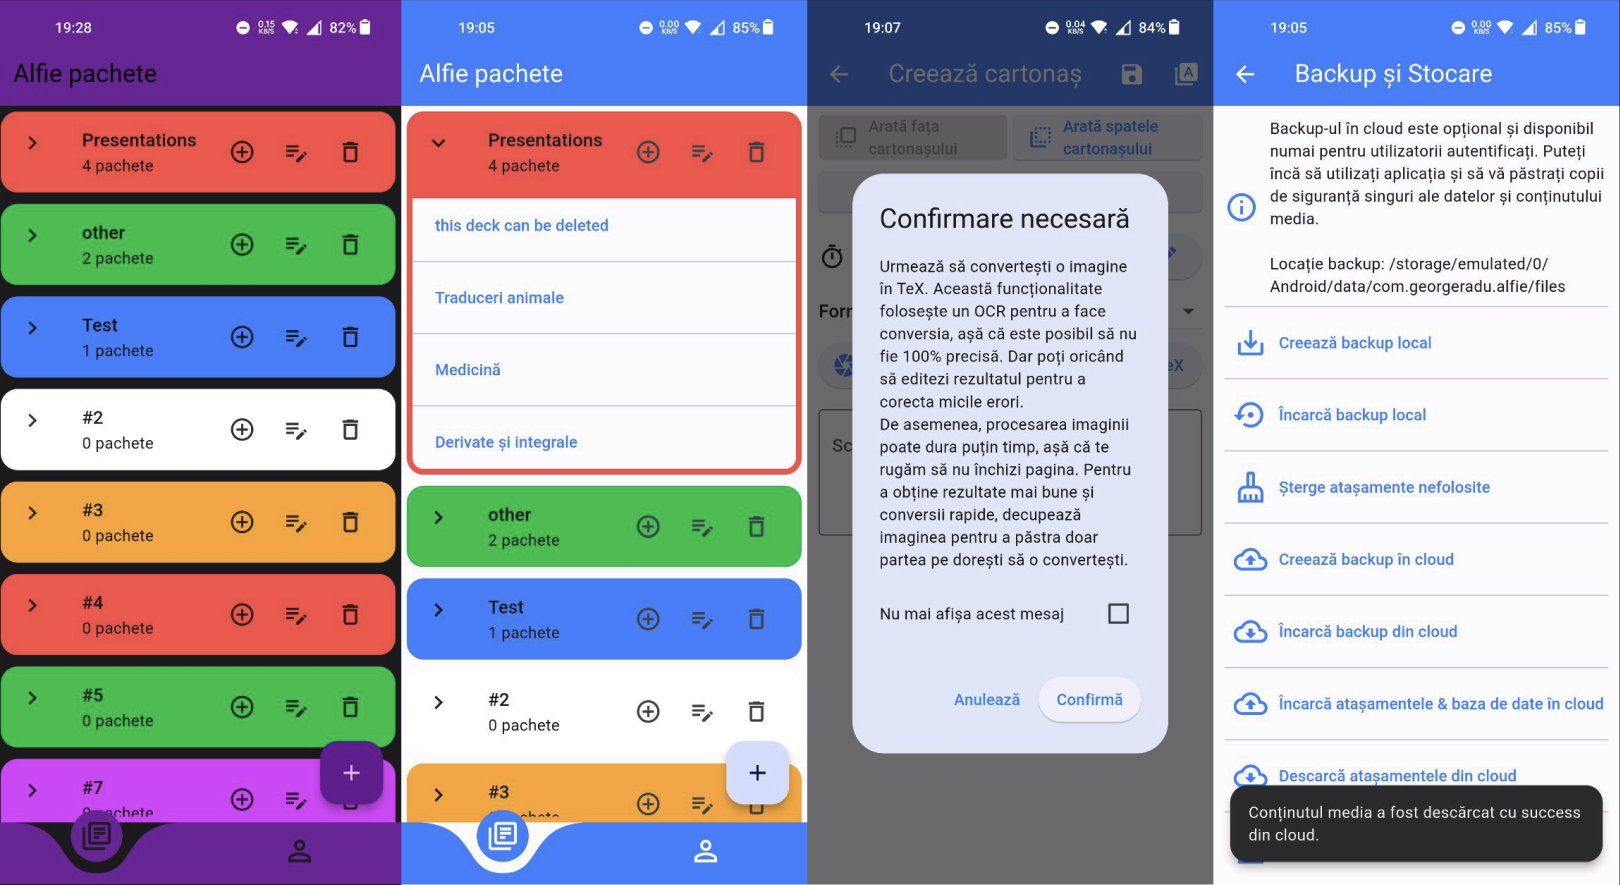
\includegraphics[width=\linewidth]{alfie-ui.png}
    \caption{Exemple de interfețe folosind 2 culori și modul de zi/noapte. Exemplu de confirmare pentru o acțiune importantă. Exemplu de informare a utilizatorului de o acțiune folosind un SnackBar}
\end{figure}

\subsection{Serviciu de permisiuni}

Diverse feature-uri ale aplicației sunt folosite de componente diferite ale telefonului mobil, cum ar fi: operații de citire și scriere pe spațiul de stocare al telefonului, accesul la internet, camera foto, galeria de conținut media a telefonului, etc. Aceste utilizări ale componentelor trebuie definite într-un fișier de configurare pentru fiecare sistem de operare în parte (Android sau iOS), astfel încât utilizatorul să fie înștiințat cu privire la permisiunile de care aplicația are nevoie pentru a rula acțiunea dorită, respectiv să-și acorde consimțământul.

Există unele permisiuni care nu necesită acordul utilizatorului, cum ar fi \textit{accesul la internet}, astfel că aplicația nu-l va mai întreba în legătură cu această permisiune, dat fiind faptul că majoritatea aplicațiilor funcționează pe baza accesului la internet, fără a avea un caracter neobișnuit sau care să invadeze privacy-ul individului.

În schimb, alte componente nu sunt necesare pentru funcționarea celor mai multor aplicații. Astfel de componente au și un caracter privat, cum ar fi \textit{accesul la camera foto} a telefonului, la \textit{galeria de conținut media} sau chiar la \textit{spațiul de stocare}. În acest caz, aplicația trebuie să ceară autorizație din partea utilizatorului pentru a accesa componentele menționate anterior.

Aplicația Alfie are nevoie de acces la camera foto și la galeria telefonului mobil pentru a obține informațiile media necesare pentru utilizarea lor în crearea de cartonașe, acolo unde utilizatorul își dorește acest lucru. De asemenea, pentru stocarea acestor imagini, generarea backup-ului local și încărcarea unui backup local, aplicația are nevoie de acces în vederea citirii și scrierii fișierelor din spațiul de stocare al telefonului. Solicitarea și aprobarea acestor tipuri de permisiuni se realizează prin crearea unui serviciu special de permisiuni care să verifice fiecare permisiune, iar în situația în care nu dispune de o permisiune, să o ceară utilizatorului.

Acțiunile care încearcă să folosească o componentă fără permisiune conduc la apariția unor erori al căror comportament nu poate fi definit. Cea mai frecvent întâlnită și deranjantă problemă introdusă este reprezentată de închiderea aplicației.

De altfel, fiecare acțiune care necesită un tip de permisiune implică o verificare a permisiunii respective, pe baza a două considerente. Pe de o parte, utilizatorul ar putea șterge oricând permisiunile unei aplicații și, pe de altă parte, telefoanele dotate cu sisteme de operare dintre cele mai noi dispun de un feature ce verifică folosirea permisiunilor de către aplicații. În cazul în care a trecut un timp îndelungat de când o aplicație nu a mai utilizat un feature, acesteia i se revocă permisiunea de a-l folosi, întrucât se consideră că nu are nevoie de el și că este cerut în mod abuziv.

\subsection{Cartonașe}

Având în vedere că principalul scop al aplicației constă în utilizarea unor cartonașe pentru a facilita procesul de învățare, în cele ce urmează acestea vor fi prezentate într-o manieră mai amănunțită. În funcție de subiectul dorit, \textbf{cartonașele} pot fi organizate în pachete, existând chiar și un feature de grupuri de pachete. Totodată, un subiect ar putea conține mai multe cartonașe, și cum este de dorit ca pachetele să nu fie foarte mari pentru a permite învățarea lor facilă, pachetele aflate sub incidența aceluiași subiect sunt grupate.

La rândul lor, grupurile pot fi customizate din punct de vedere cromatic, folosind mai multe culori de fundal, iar pachetele pot fi mutate dintr-un grup în altul. Opțiunea de ștergere a unui grup ce conține pachete de cartonașe este indisponibilă, astfel încât să fie evitate pierderile de date în mod neintenționat. În schimb, pachetele pot fi șterse doar după o reconfirmare într-un dialog de alertă, întrucât cartonașele conținute de acestea vor fi șterse, de asemenea. Pachetele conțin un field pentru nume, precum și o descriere extinsă, care să permită utilizatorului salvarea scopului deck-ului respectiv. Acest feature se dovedește extrem de util în cazul utilizatorilor ce și-au creat mai multe pachete pentru organizare.

În meniul de pachete pot fi adăugate cartonașe noi. Un cartonaș este compus din două fețe: prima față cuprinde întrebarea, iar a doua față ilustrează răspunsul aferent.

Sunt implementate 3 tipuri de cartonașe:
\begin{enumerate}
    \item \textbf{cartonașe simple} - după cum sugerează și numele, acestea reprezintă cele mai simple cartonașe, fiind alcătuite doar din cele două fețe;
    \item \textbf{cartonașe cu răspuns type in} - acest tip de cartonașe vine cu opțiunea de a scrie răspunsul în modul de studiu atunci când se efectuează revizuirea. La final se poate observa atât întrebarea și răspunsul acordat în modul de studiu, cât și răspunsul adevărat al întrebării de pe cartonaș;
    \item \textbf{cartonașe de tip quizz} - sunt formate dintr-o întrebare și mai multe opțiuni de răspuns (între 3 și 8 variante). În modul de studiu va fi prezentată întrebarea și lista de opțiuni, iar atunci când utilizatorul va alege o opțiune, adevăratul răspuns va fi afișat.
\end{enumerate}

Un alt feature pe care îl au toate tipurile de cartonașe constă în \textit{setarea unui timer}. În felul acesta, utilizatorul este constrâns să răspundă într-un anumit interval de timp la fiecare întrebare. În modul de studiu, dacă utilizatorul nu răspunde suficient de rapid, i se va afișa răspunsul automat. Totodată, în modul de studiu, utilizatorul va vedea dacă un cartonaș are sau nu setat un interval pentru a răspunde și, totodată, cât timp i-a rămas până la afișarea răspunsului.

Cartonașele oferă 4 tipuri de formatări de text, și anume:
\begin{enumerate}
    \item \mintinline{tex}{Simplu} - nicio formatare specială, fiind eficientă în cazul întrebărilor scurte întrucât se încarcă cel mai rapid;
    \item \mintinline{tex}{Markdown} - oferă suport pentru afișare în formatul Markdown combinat cu HTML (cel mai folosit pentru styling); suport pentru ecuații și expresii matematice, fizice, chimice;
    \item \mintinline{tex}{TeX} - oferă suport pentru afișare în formatul TeX. Motorul de randare este Katex.
    \item \mintinline{tex}{HTML} - este utilizat ca opțiune pentru mai multe customizări de cartonașe și styling considerat mai ușor.
\end{enumerate}

De asemenea, cartonașele au implementată opțiunea de a adăuga imagini atât pe partea cu întrebarea, cât și pe cea de răspuns. Imaginile adăugate pot fi preluate atât din galeria de imagini, cât și folosind camera foto a telefonului mobil. După selectarea imaginii, utilizatorul are posibilitatea de a o edita în funcție de scopul pe care și l-a propus. În acest sens, sunt disponibile opțiuni de decupare, adăugare de text, marker pentru evidențierea unor zone. Prin acest feature, cartonașele aduc mai multe customizări pentru utilizatorul final.

\begin{figure}[H]
    \centering
    \textbf{Exemple de cartonașe în aplicația Alfie}\par\medskip
    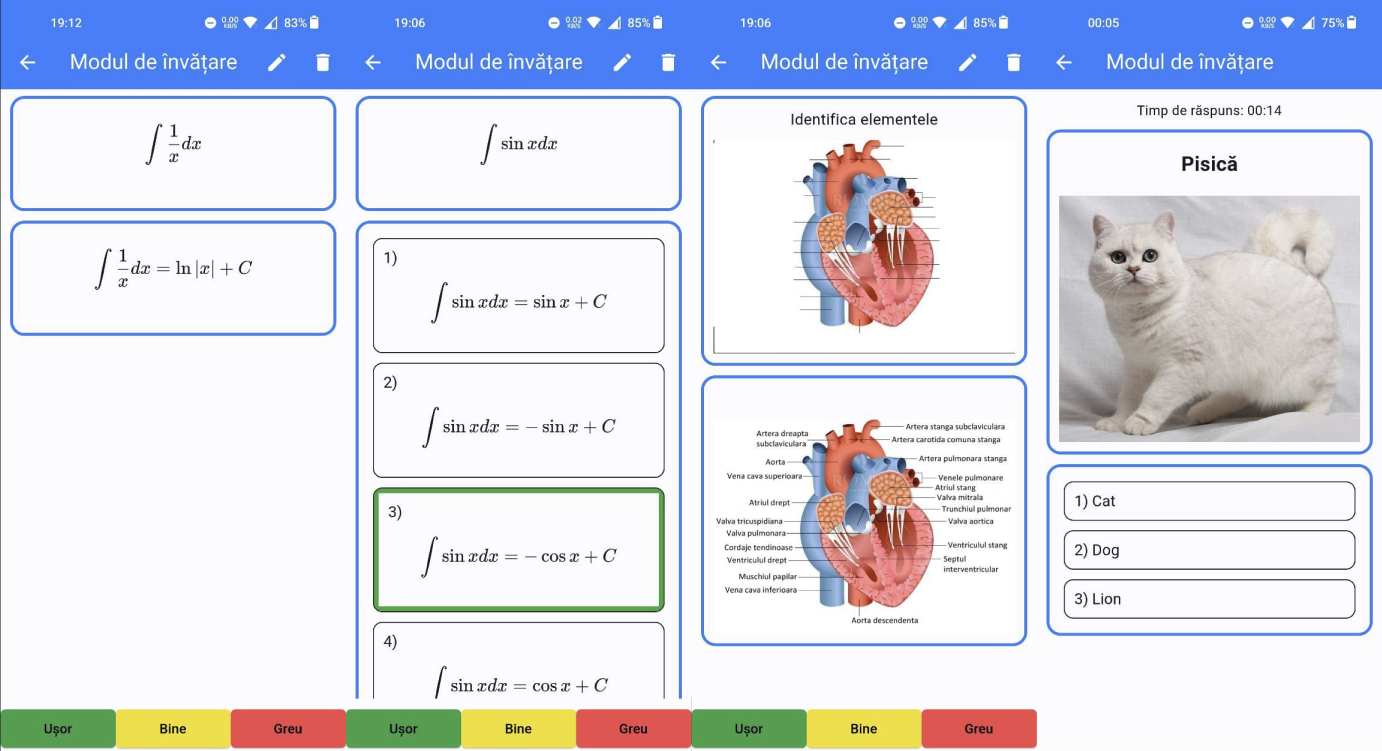
\includegraphics[width=\linewidth]{alfie-cartonase.png}
    \caption{Exemplu de cartonaș simplu care conține text științific. Exemplu de cartonaș de tip quizz cu text științific. Exemplu de cartonaș având conținut media. Exemplu de cartonaș de tip quizz care conține o imagine și are timp limită de răspuns.}
\end{figure}

Cartonașele care se folosesc de formatarea TeX beneficiază și de un feature de OCR, care este valabil doar în cazul utilizatorilor logați în cont. Acest feature le oferă capabilitatea de a fotografia o expresie matematică și de a o obține sub format TeX. Detalii despre implementarea acestui serviciu vor fi prezentate ulterior.

După obținerea rezultatului, utilizatorul are opțiunea de a-l modifica dacă dorește acest lucru sau de a-l corecta, în cazul greșelilor minore. În cazul în care OCR-ul înregistrează o precizie mică, acesta îi va solicita utilizatorului să reia procesul și să ofere o imagine mai clară.

\subsection{Modul de studiu}

În meniul unui pachet de cartonașe se află meniul de studiu, ce va prezenta, pe rând, fața unui cartonaș pe care este afișată întrebarea. Utilizatorul va alege un răspuns, acțiune care va prezenta și fața ce include răspunsul corect al cartonașului. În continuare, utilizatorul are opțiunea de a selecta nivelul de dificultate al cartonașului folosind una dintre cele trei metrici (ușor, mediu, greu). De asemenea, în cazul cartonașelor care au setat un interval limită pentru răspuns, se folosește un timer ce afișează în timp real timpul scurs până la afișarea automată a răspunsului corect.

După afișarea răspunsului unui cartonaș, utilizatorul obține acces la încă două opțiuni pentru cartonaș. Prima opțiune este cea de editare a cartonașului, în cazul apariției anumitor greșeli la crearea acestuia de către utilizator. Opțiunea de editare va deschide un meniu similar cu cel de creare a cartonașului ce va conține datele introduse inițial pe cartonaș, astfel încât să poată fi editate în mod direct. Cea de-a doua opțiune este cea de ștergere a cartonașului, cu dublă confirmare printr-un dialog de alertă. Această opțiune îi permite utilizatorului să șteargă cartonașele pe care le consideră irelevante pentru pachetul respectiv.

În modul de studiu, cartonașele unui pachet sunt prezentate utilizatorului în funcție de relevanță. Prin această \textbf{relevanță} se înțelege gradul de dificultate întâmpinat de utilizator la fiecare cartonaș în parte și momentul în care trebuie să fie reverificat.

Pentru sortarea cartonașelor în funcție de această metrică se folosește o coadă de prioritate cu structură de tip heap. Heap-ul este o structură de tip matrice care poate fi văzut drept un arbore binar aproape complet, unde fiecare nod din arbore corespunde unui element din matrice. Aplicația utilizează un max-heap, dat fiind faptul că proprietatea max-heapului este aceea că pentru fiecare nod cu excepția rădăcinii, valoarea nodului părinte este mai mare decat valoarea nodului. Astfel, structura de date va fi sortată în funcție de scorul cel mai mare. Printre proprietățile care favorizează această structură de date ca fiind o alegere bună pentru a fi folosită drept o coadă de priorități eficientă se numără faptul că inserările și extragerea rădăcinii se realizează în timp logaritmic $\mathcal{O}(\lg n)$ \cite{introductionAlgorithms}.

Fiecărui cartonaș îi este asignat un scor pentru această metrică, scor care va fi folosit de coada de prioritate pentru compararea lor. Calcularea scorului unui cartonaș este determinată de un algoritm intern ce combină mai multe metrici, precum: timpul de la ultimul review, ultimul rating și numărul de review-uri. Cartonașul primește câte un punct pentru fiecare zi de la ultimul review. În cazul în care cartonașul nu a fost revizuit se va considera data de la ultima actualizare. În funcție de ultimul rating al cartonașului se vor adăuga puncte pe baza gradului de dificultate atribuit cartonașului de către utilizator. De asemenea, pentru fiecare nivel de dificultate se vor scădea puncte dacă nu a trecut suficient timp de la ultimul review. În cazul unui cartonaș evaluat ca fiind „ușor” se va aplica o penalizare pentru un review care nu este mai vechi de 7 zile, pentru un cartonaș considerat „mediu”, intervalul limită de timp este de doar 2 zile, iar în cazul ultimului nivel de dificultate („greu”), penalizarea se aplică după 2 ore. Cartonașele care nu au fost revizuite vor primi un scor semnificativ în plus pentru a putea fi revizuite. Altfel, scăderea punctelor aferente fiecărui cartonaș se face liniar, în funcție de numărul de review-uri. La final, se mai adaugă un scor din intervalul [−20,20] pentru a schimba în mod aleator ordinea cartonașelor ce prezintă un rating similar, dar care să nu afecteze celelalte metrici.

\subsection{Statistici pentru învățare}

Pentru motivarea utilizatorului în procesul său de învățare este oferită o pagină de \textbf{statistici} privind rezultatele obținute și progresul acestuia în timp real.

Pagina de statistici conține trei diagrame configurabile în funcție de timeline-ul review-urilor (tot timpul, ultima săptămână, ultima lună, ultimul semestru):
\begin{enumerate}
    \item un \textit{pie-chart} pentru a ilustra sub formă procentuală rezultatele obținute;
    \item un \textit{timeline} pentru a reda progresul înregistrat în perioada selectată;
    \item un \textit{barline} pentru a ilustra rapiditatea de răspuns la cartonașe.
\end{enumerate}

Exemple de aceste diagrame se pot găsi în figurile \ref{fig:statistici_1} și \ref{fig:statistici_2} de mai jos.

\begin{figure}[H]
    \centering
    \textbf{Statistici procentuale pentru ratingul cartonașelor}\par\medskip
    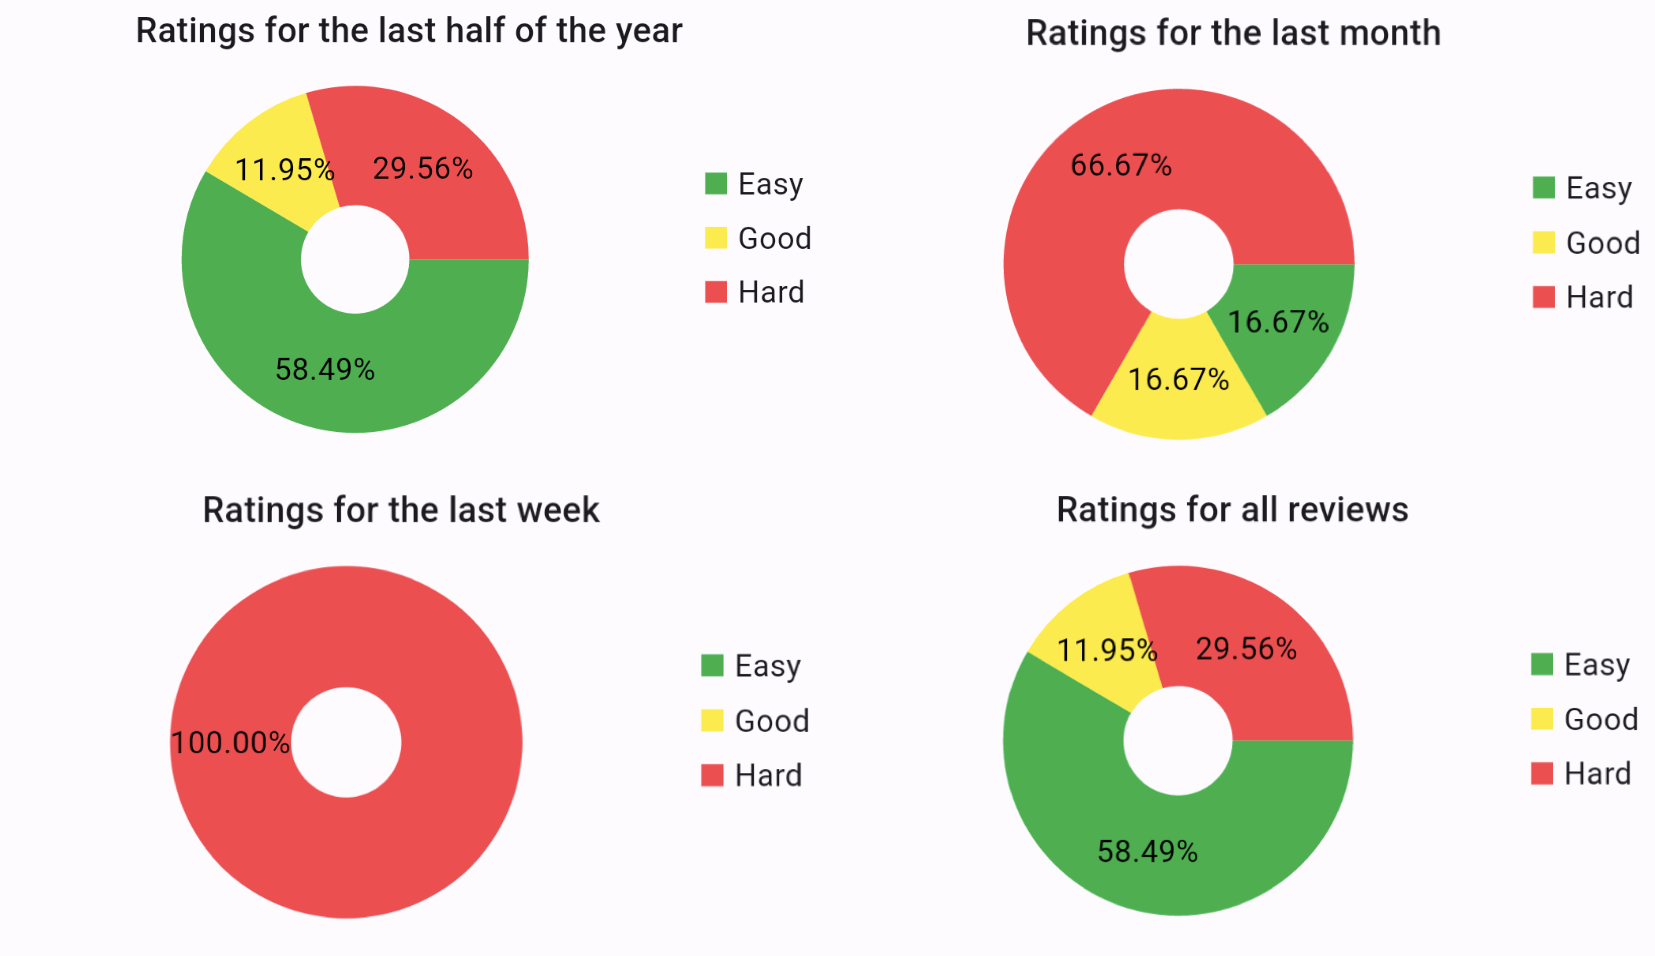
\includegraphics[width=.7\linewidth]{statistics-piechart.png}
    \caption{Statistici sub formă de pie-chart pentru 4 timeline-uri}
    \label{fig:statistici_1}
\end{figure}

\begin{figure}[H]
    \centering
    \textbf{Statistici în timp pentru ratingul cartonașelor}\par\medskip
    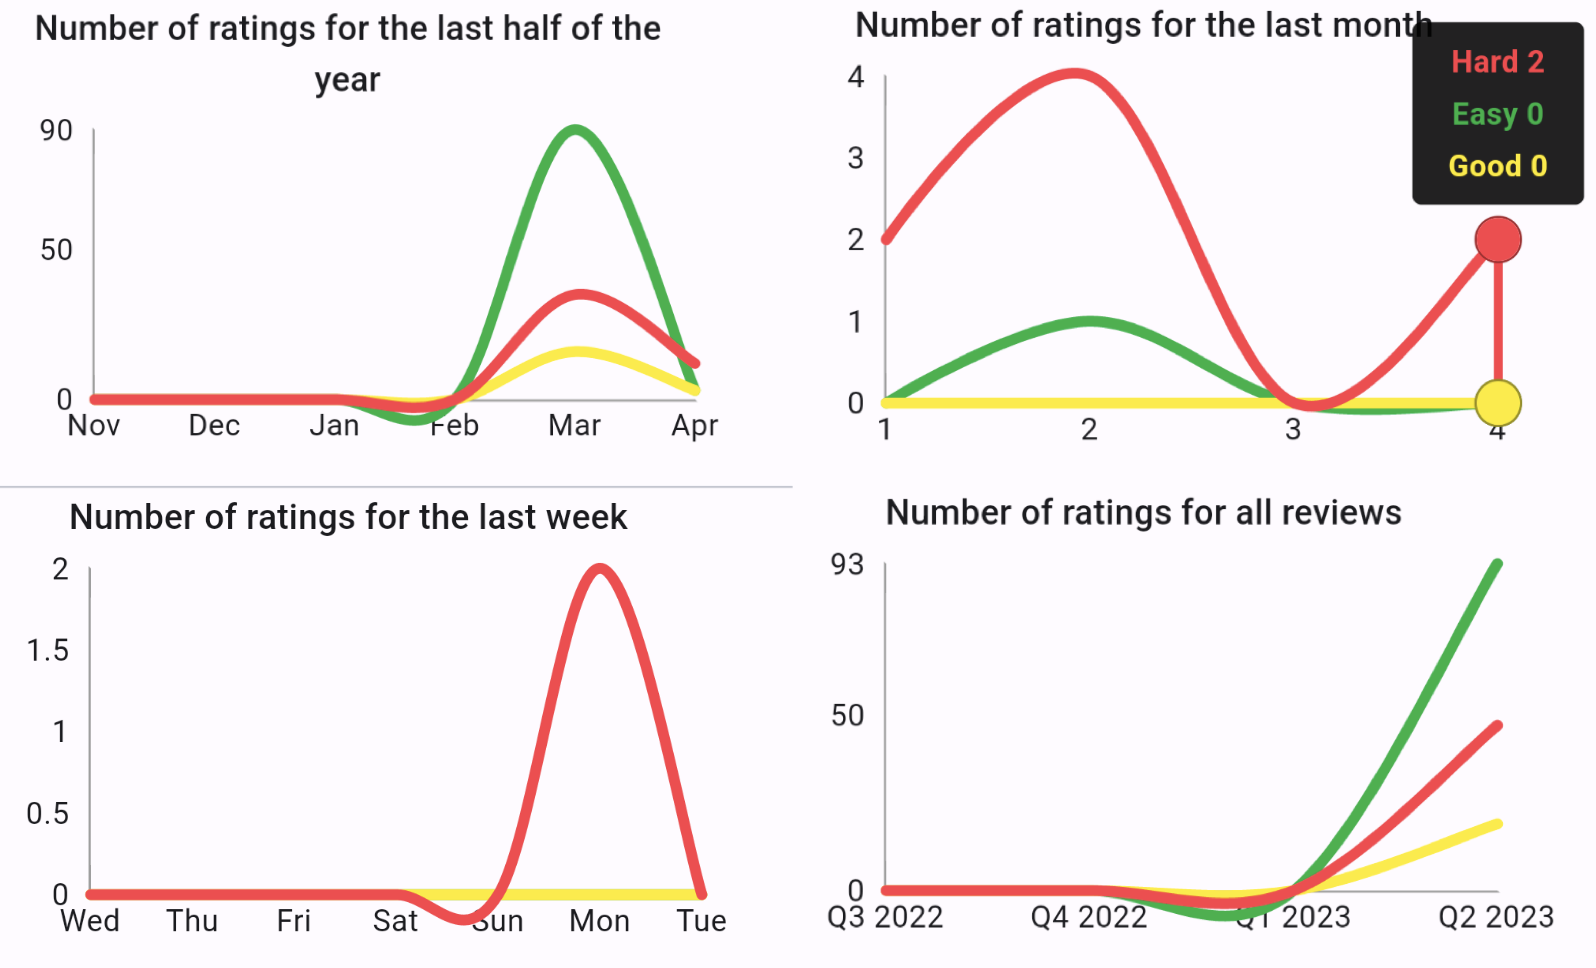
\includegraphics[width=.7\linewidth]{statistics-timeline.png}
    \caption{Statistici sub formă de timeline pentru 4 timeline-uri}
    \label{fig:statistici_2}
\end{figure}

\subsection{Backup și Storage local}

Aplicația oferă două opțiuni de backup. Prima opțiune este cea care creează backup pentru cartonașe în spațiul de stocare al telefonului. Conținutul media este salvat tot local, pentru a fi accesibil utilizatorului. În felul acesta, utilizatorul își transferă fișierele și le salvează în mod independent, fără a fi nevoie să-și creeze un cont Alfie.

În schimb, utilizatorii care folosesc un cont Alfie beneficiază și de opțiunea de backup în cloud atât a bazei de date cu cartonașe cât și a întregului conținut media. De asemenea, acest tip de backup poate fi descărcat oricând la nevoie. Conținutul media descărcat va fi doar cel care lipsește local și poate fi recuperat din cloud.

Este important de menționat faptul că aplicația păstrează și conținutul media vechi. Cu alte cuvinte, conținutul media înlocuit în momentul actualizării unui cartonaș continuă să fie păstrat în cloud pentru a putea fi refolosit de utilizator în cazul în care noul conținut nu se potrivește cartonașului respectiv. Pentru a satisface și cererea utilizatorilor care nu doresc să păstreze conținutul media nefolosit de cartonașe există și o opțiune de ștergere definitivă a acestuia.

În aceeași pagină există, totodată, și opțiunea de ștergere a review-urilor mai vechi acordate cartonașelor, în funcție de perioada de timp. În felul acesta, utilizatorul eliberează spațiul de stocare și elimină review-urile vechi ale cartonașelor care, probabil, nici nu mai sunt de actualitate.

\section{Backend - api in Go}

\subsection{Go}

Go este un limbaj de programare open source și versatil, dezvoltat de Google, fiind utilizat în majoritatea organizațiilor gigant (cum ar fi: Google, CapitalOne, CloudFlare, Meta, Microsoft, Salesforce, Uber) pentru rularea serviciilor \cite{goDev}. Go este considerat un limbaj ușor de învățat și foarte eficient în cazul echipelor, după cum menționează Jaime Enrique Garcia Lopez, Senior Software Development Manager at Capital One \cite{goDev}.

Unul dintre avantajele faptului că este un limbaj open source și foarte popular este acela că are un ecosistem mare, unelte și librării, pe lângă cea standard \cite{goSTDLibrary}, precum una de criptografie care conține și algoritmi criptografici noi \cite{goCryptoModule}. Go poate compila toate librăriile și modulele într-un singur binar pentru fiecare sistem de operare și arhitectură. De asemenea, Go folosește un sistem de tipuri statice și are o amprentă mică pe memorie cu un rol foarte important în cazul aplicațiilor mari \cite{goDevMatt}.

Compilatorul de Go poate crea build-uri de programe rapid \cite{goCLIs}, care rulează pe orice sistem \cite{goReleases}. Go este foarte extensibil, putând fi utilizat pentru servicii de cloud și rețele \cite{goCloud}, la interfețe pentru linia de comandă \cite{goCLIs}, respectiv la dezvoltarea aplicațiilor web \cite{goWebDev}.

\subsubsection{De ce este folosit în Alfie?}

Pentru usecase-ul aplicației Alfie se folosește Go în vederea construirii unui api, întrucât oferă un suport excelent pentru ultimele tehnologii, cum ar fi: HTTP/2, drivere pentru baze de date, ORM-uri, dar și ultimele standarde de criptare \cite{goWebDev}. Totodată, faptul că are o interfață CLI este de un real ajutor pentru config-ul de Docker, alături de avantajul de a suporta multe librării open source. Un alt avantaj în procesul de dezvoltare constă în faptul că Go este static typed.

\subsubsection{Particularități ale limbajului}

Go nu se folosește de clase \cite{goByExample}. Pentru a grupa datele sau pentru a construi tipuri de record-uri, acesta oferă conceptul de struct-uri, care reprezintă o colecție de field-uri definite cu tipuri \cite{goByExampleStructs}. Peste aceste struct-uri pot fi stabilite metode \cite{goByExampleMethods}, precum cele din exemplul de cod sursă nr. \ref{code:go_structs_and_methods}.

\begin{code}
    \inputminted[frame=single,framesep=2mm,linenos,breaklines,tabsize=2]{go}{code/go-structs.go}
    \captionof{listing}{Exemplu de structuri și metode în Go}
    \label{code:go_structs_and_methods}
\end{code}

Pentru abstractizarea structurilor, Go oferă conceptul de interfețe \cite{goByExampleInterfaces}. În acest sens, pot fi folosite diverse obiecte după o structură bine definită a funcțiilor ce au interfețe drept parametrii sau care returnează interfețe. Dacă structura nu implementează toate metodele interfeței programul nu va putea fi compilat. Conceptul de interfețe este similar din acest punct de vedere cu alte limbaje de programare care îl implementează. Un exemplu pentru interfețe este redat în codul sursă nr. \ref{code:go_interfaces}.

\begin{code}
    \inputminted[frame=single,framesep=2mm,linenos,breaklines,tabsize=2]{go}{code/go-interfaces.go}
    \captionof{listing}{Exemplu de interfețe in Go}
    \label{code:go_interfaces}
\end{code}

De asemenea, Go suportă încorporarea de struct-uri și interfețe pentru a realiza o compoziție mai ușoară a tipurilor \cite{goByExampleStructEmbedding}. Din moment ce Go nu admite conceptul de clase sau moștenire, conceptul de compoziție este ca o trăsătură a paradigmei orientate obiect, după cum este ilustrat în codul sursă nr. \ref{code:go_structs_embedding} de mai jos.

\begin{code}
    \inputminted[frame=single,framesep=2mm,linenos,breaklines,tabsize=2]{go}{code/go-struct-embedding.go}
    \captionof{listing}{Exemplu de compoziție în Go}
    \label{code:go_structs_embedding}
\end{code}

\subsection{PostgreSQL \& GORM}

PostgreSQL este o bază de date relațională open source. Fiind considerată o bază de date relativă, aceasta se află în dezvoltare activă de 35 de ani, motiv pentru care a câștigat o reputație bună în ceea ce privește integritatea datelor și extensibilitate \cite{postgresqlAbout}.

Printre principalele avantaje ale PostgreSQL se numără atât faptul că rulează pe toate sistemele mari de operare \cite{postgresqlSupportedPlatforms}, cât și că recuperează datele în caz de dezastre, folosind diferite metode (write ahead loggings, replication, point in time recovery) \cite{postgresqlAbout}.

Un alt factor important în alegerea unei baze de date este conformarea cu proprietățile ACID, factor valabil și în cazul PostgreSQL.

În ceea ce privește feature-urile acestei baze de date, merită menționată existența multiplelor tipuri de date, pe lângă cele deja cunoscute (primitive, structuri, documente, dar având și opțiunea de a adăuga propriile tipuri custom).

Pentru comunicațiile dintre api-ul în Go și baza de date PostgreSQL, aplicația de Go se folosește de ORM-ul GORM. Principalele motive ce stau la baza alegerii acestui ORM sunt \cite{gormOverview}:
\begin{enumerate}
    \item suport pentru \textit{asociații între modele} (one-to-one, one-to-many, many-to-many);
    \item suport pentru \textit{tranzacții} și \textit{save points} – un motiv important din moment ce a fost aleasă baza de date PostgreSQL pentru conformitatea cu principiile ACID;
    \item conectarea la baza de date și suportul oferit pentru \textit{migrații ale modelelor}, în trecerea de la o versiune la alta (prin migrații automate este seamingless \ref{code:go_connect_database_and_migrations});
    \item \textit{construcție robustă}, în care fiecare feature dispune de teste de implementare \cite{gormTest};
    \item \textit{declararea modelelor și a proprietăților field-urilor} este realizată foarte simplu cu sintaxa de Go, precum în exemplul \ref{code:go_user_model_gorm}.
\end{enumerate}

\subsection{gRPC}

\textbf{gRPC} este un framework pentru apelurile de proceduri la distanță (RPC), ce poate fi folosit împreună cu 11 limbaje de programare \cite{grpcFAQ}. gRPC este un proiect din cadrul Cloud Native Computing Foundation încă din data de 16 Februarie 2017 \cite{grpcCNCF}, fiind utilizat cu succes de companii, precum: Square, Netflix, CoreOs, Cisco \cite{grpcIO}.

Printre motivele utilizării gRPC în proiectul \textit{Alfie}, se numără:
\begin{enumerate}
    \item posibilitatea de a dezvolta o aplicație pentru clienții de mobil care trebuie să comunice cu un server;
    \item design-ul stratificat ce suportă autentificare, load balance, logging și monitorizare;
    \item protocolul este eficient și independent de limbaj;
    \item permite o dezvoltare mai eficientă, întrucât expune clientului metodele ce pot fi suportate de server, parametrii pe care trebuie să îi trimită și tipurile de date la care să se aștepte drept răspuns, alături de posibilele erori;
    \item framework-ul este static typed;
    \item oferă suport de streaming bidirecțional și este integrat cu transport de tip HTTP/2.
\end{enumerate}

gRPC apelează la \mintinline{tex}{protocol buffers} pentru definiția limbajului și schimbul de mesaje, bazându-se pe ideea unei definiții de serviciu în care se specifică metodele, parametrii și tipurile returnate.

\begin{code}
    \inputminted[frame=single,framesep=2mm,linenos,breaklines,tabsize=2]{protobuf}{code/exemplu-serviciu.proto}
    \captionof{listing}{Exemplu de definiție a unui serviciu folosind gRPC}
    \label{code:grpc_service_example}
\end{code}

Serverele vor implementa interfața \mintinline{protobuf}{Alfie} ilustrată în codul sursă nr. \ref{code:grpc_service_example} și vor rula un server de gRPC pentru a asculta apelurile de la client. Așadar, utilizatorii vor avea un stub (client) care va expune aceleași metode ca și cele definite pe server de serviciul \mintinline{protobuf}{Alfie}.

În acest caz, pe server va fi implementată \textit{interfața} oferită de serviciul Alfie cu o metodă \mintinline{protobuf}{HelloWorld} ce va primi drept parametru \mintinline{protobuf}{HelloWorldRequest} și va întoarce un tip \mintinline{protobuf}{HelloWorldReply}, având posibilitatea de a genera erori (sau a returna și o eroare, în funcție de limbajul de programare ales).

Tipurile parametrilor și a valorilor returnate se definesc în același fișier și sunt static typed. Mesajele reprezintă record-uri care conțin informații, precum: tip/nume/valoare/ordine, numite field-uri. Pot fi folosite \textit{tipuri clasice}, cum ar fi: \mintinline{protobuf}{string}, \mintinline{protobuf}{int64}, \mintinline{protobuf}{bool}, dar se pot construi și liste cu ajutorul cuvântului cheie: \mintinline{protobuf}{repeatead}. De asemenea, se pot defini și tipuri noi \textit{pe baza mesajelor construite}, precum \mintinline{protobuf}{SimpleMessage}, care este folosit în calitate de tip al unei liste în mesajul \mintinline{protobuf}{HelloWorldReply} (redat în codul sursă nr. \ref{code:grpc_message_example}).

\begin{code}
    \inputminted[frame=single,framesep=2mm,linenos,breaklines,tabsize=2]{protobuf}{code/exemplu-mesaje.proto}
    \captionof{listing}{Exemple de tipuri de mesaje ce pot fi definite}
    \label{code:grpc_message_example}
\end{code}

În cazul acestui proiect va fi aplicată versiunea 3 de protocol buffers (proto3), ținând cont de faptul că dispune de o sintaxă simplificată și suportă mai multe limbaje de programare \cite{grpcIntro}.

Serviciul \mintinline{protobuf}{Alfie} din codul sursă nr. \ref{code:grpc_alfie_service}, ce este definit pentru comunicații între serverul în Go și clientul de Dart, conține următoarele endpoint-uri:

\begin{code}
    \inputminted[frame=single,framesep=2mm,linenos,breaklines,tabsize=2]{protobuf}{code/alfie-service.proto}
    \captionof{listing}{Definitie servciu Alfie folosind Protobuf}
    \label{code:grpc_alfie_service}
\end{code}

După definirea serviciului dorit în gRPC trebuie generat codul pentru server și client. În acest sens, va fi utilizat compilatorul de protocol buffers \mintinline{shell}{protoc}, împreună cu extensiile sale, astfel încât să genereze codul pentru Go și Dart. Comenzile necesare la compilare sunt definite în codul sursă nr. \ref{code:generate_grpc} de mai jos.

\begin{code}
    \inputminted[frame=single,framesep=2mm,linenos,breaklines,tabsize=2]{bash}{code/generate-grpc.sh}
    \captionof{listing}{Generarea codului pentru serverul în Go și clientul de Dart din serviciul Alfie definit cu gRPC}
    \label{code:generate_grpc}
\end{code}

\subsection{Structura api}

În funcție de rolurile ce îi sunt atribuite, Api-ul este structurat în următoarele directoare:

\begin{enumerate}
    \item \textbf{config} -  conține fișiere de configurare pentru variabilele de environment, configurarea serverului de gRPC și conectarea la baza de date;
    \item \textbf{protobuf} - conține fișierul .proto pentru definirea serviciului și fișierele .go generate folosind compilatorul protos;
    \item \textbf{delivery} - va conține implementarea serviciului Alfie definit în protobuf;
    \item \textbf{models} - conține fișierele cu modelele definite ale aplicației, folosind struct-uri de go și extensia de gORM;
    \item \textbf{repository} - conține layer-ul pentru acces la baza de date, respectiv interfața de repository cu implementare, fiecare model fiind localizat în propriul său fișier;
    \item \textbf{services} - conține interfețele și implementările pentru servicii, cum ar fi cel de JWT și cele 3rd api, precum \textit{verificare mail} (cu implementare folosind twilio), \textit{media cloud} (cu implementare folosind S3) și unul de \textit{validare a datelor};
    \item \textbf{usecase} - conține managerele care se vor ocupa de cererile utilizatorilor apelând celelalte servicii și repository;
    \item \textbf{utils} - conține iteme utile, precum cel de logging, pentru informații și erori.
\end{enumerate}

\subsection{Serviciu pentru validarea datelor}

Proiectul este structurat de așa manieră încât să existe două tipuri de validare a datelor:
\begin{enumerate}
    \item O primă validare realizată \textit{la nivel de client} pentru a-l îndruma pas-cu-pas în utilizarea aplicației și, respectiv, pentru salvarea datelor valide;
    \item O a doua validare realizată \textit{la nivel de server} pentru a asigura salvarea informațiilor corecte și valide. Deși sunt realizate validări la nivel de client înainte de a interacționa cu serverul, acesta nu trebuie să se bazeze pe respectivele validări, dat fiind faptul că serverul ar putea primi cereri și din partea altor clienți în afară de aplicația de mobil, neputând fi controlați nici clienții, nici validitatea datelor trimise de către aceștia.
\end{enumerate}

Așadar, pentru aplicația de Go este definită o interfață a serviciului de validare a datelor, ce conține metodele care trebuie implementate pentru asigurarea validității tuturor datelor primite.

\subsection{Autentificare}

Pentru autentificarea utilizatorilor, \textit{Alfie} folosește un serviciu de tip \mintinline{go}{JWT}. Interfața acestuia este simplă, solicitând două implementări de funcții: una pentru crearea tokenului și una pentru validarea acestuia, așa cum este ilustrat în codul sursă nr. \ref{code:go_jwt_service}. În procesul de implementare, serviciul de \mintinline{go}{JWT} apelează librăria de \mintinline{go}{jwt} pentru go. Emailul utilizatorului este definit drept claim adițional al tokenului. În ceea ce privește configurarea serviciului, acesta utilizează două valori de environment, și anume: una pentru cheia secretă care va genera tokenii și una pentru a seta valabilitatea unui token.

\begin{code}
    \inputminted[frame=single,framesep=2mm,linenos,breaklines,tabsize=2]{go}{code/jwt-service.go}
    \captionof{listing}{Interfața pentru serviciul JWT în Go}
    \label{code:go_jwt_service}
\end{code}

De altfel, pentru autentificare api-ul de go folosește un interceptor unar pentru serverul de gRPC. Interceptorul unar are acces la serviciul \mintinline{go}{JWTService} și la o mapă de rute (rpc-uri) care nu au nevoie de autentificare, cea din urmă fiind mai ușor de întreținut. Datorită faptului că majoritatea rpc-urilor sunt autentificate, la adăugarea unei noi rute, un client ar putea să omită inserarea acesteia și în lista respectivă. În schimb, o nouă rpc dezvoltată este mai ușor de detectat atunci când nu are nevoie de autentificare întrucât, dacă nu este adăugată în mapping, aceasta va fi tratată ca și cum ar avea nevoie de autentificare, lucrul acesta putând fi observat imediat în log-uri.

Token-ul este preluat din contextul apelului și este validat folosind \mintinline{go}{JWTService}. Dacă nu este valid atunci va întoarce un răspuns pentru a informa apelantul că nu este autorizat. În cazul în care token-ul este valid, interceptorul va trimite mai departe email-ul userului din claimurile token-ului, astfel încât metodele autorizate să aibă acces la cine a apelat rpc-ul și, totodată, certitudinea că este un claim valid.

În procesul de autentificare al utilizatorilor este setată, în mod implicit, și opțiunea de 2FA pentru logarea prin email. Astfel, în momentul logării, utilizatorul se va conecta prin email și parolă, iar în baza de date se va marca atât că poate avea loc verificarea 2FA, cât și timestamp-ul la care a început logarea. Următorul pas este de a trimite utilizatorului un cod de verificare 2FA pe adresa de email furnizată, apelând la serviciul de mail. În continuare, utilizatorul are la dispoziție 10 minute pentru a se loga cu 2FA. La expirarea intervalului de timp setat, acesta va fi nevoit să reia întregul proces.

De asemenea, în cazul în care își uită parola, dar are acces la email, utilizatorul va putea să-și reseteze parola, primind în acest sens un cod de verificare pe adresa de email înregistrată care va fi folosit pentru verificarea deținerii titlului de proprietar al contului, respectiv pentru setarea unei noi parole.

\subsection{Securitatea parolelor}

Pentru salvarea parolelor utilizatorilor, acestea vor fi hashuite înainte de salvare. Algoritmul de hash folosit este \mintinline{go}{Argon2id}. Argon este câstigătorul competiției Password Hashing, ce a fost organizată în perioada 2013-2015 \cite{passwordHashingCompetition}. Competiția a fost una deschisă, similară cu cele organizate de NIST pentru \mintinline{tex}{AES} și \mintinline{tex}{SHA-3} \cite{passwordHashingCompetition}, având scopul de a stabili un nou standard pentru generarea hash-urilor parolelor din aplicațiile moderne.

Algoritmul Argon a fost creat de Alex Biryukov, Daniel Dinu și Dmitry Khovratovich de la Universitatea Luxemburg. Totodată, Argon2id este algoritmul pentru hashing de parole recomandat de OWASP \cite{owaspPasswordHashing}.

Ținând cont de aceste considerente, Alfie folosește implementarea în Go din packetul crypto \cite{goXCrypto} pentru \mintinline{go}{argon2}.

\begin{code}
    \inputminted[frame=single,framesep=2mm,linenos,breaklines,tabsize=2]{go}{code/hash-password.go}
    \captionof{listing}{Crearea unui hash pentru o parolă}
    \label{code:go_hash_password}
\end{code}

La generarea hash-ului unei parole este utilizat conceptul de \textbf{salting}, care determină un salt unic pentru fiecare utilizator în parte, cu ajutorul unui generator criptografic de numere aleatoare \cite{goCryptographicRNG}. Generatorul criptografic ales provine din librăria standard de Go. Librăria folosește pentru fiecare sistem de operare generatorul criptografic pus la dispoziție \cite{goCryptographicRNG}. Așadar, parola utilizatorului va fi hash-uită împreună cu un salt unic, fiind creat în acest sens un hash diferit pe același input de parolă, dat fiind faptul că va fi generat un alt salt (probabilitate neglijabilă să fie același).

\begin{code}
    \inputminted[frame=single,framesep=2mm,linenos,breaklines,tabsize=2]{go}{code/generate-salt.go}
    \captionof{listing}{Generarea salt-ului pentru hashing-ul de parole folosind un generator de numere aleatoare criptografic}
    \label{code:go_generate_salt}
\end{code}

Salt-ul și hash-ul parolei aferente fiecărui utilizator vor fi salvate în baza de date. Astfel, în momentul autentificării, api-ul va genera hash-ul pentru parola din cerere împreună cu salt-ul din baza de date și va verifica să fie același rezultat cu hash-ul parolei salvat în db pentru logare.

În felul acesta, aplicația \textit{Alfie} se conformează la noile standarde pentru securitate propuse de specialiștii în domeniu.

\subsection{Integrare mail cu Twilio și SendGrid}

Twilio reprezintă unul dintre standardele de verificare a utilizatorilor, ce permite foarte multe canale de comunicare (SMS, WhatsApp, Email, voce, Push, TOTP) \cite{twilioAuthChannels}. Twilio SendGrid reprezintă serviciul de mail oferit de Twilio.

Proiectul Alfie folosește Twilio cu scopul de a verifica conturile utilizatorilor care apelează la serviciile Alfie din cloud, dar și pentru a oferi protecție 2FA implicită. Serviciul de verificare aplicat este cel prin email, iar cel de 2FA dispune și de rolul de resetare al parolei. În \cite{twilioEmail2FATradeoffs}, Kelley Robinson dezbate dacă canalul de email este unul sigur pentru 2FA, însă acest lucru variază și în funcție de usecase-ul aplicației. În cazul utilizatorilor Alfie, verificarea prin email reprezintă o metodă eficientă de a proteja conturile utilizatorilor, în special datorită faptului că aplicația nu presupune cerințe de securitate națională.

Prin intermediul Twilio SendGrid sunt customizate trei template-uri de mailuri, și anume: mail pentru verificarea înregistrării unui utilizator, mail pentru resetarea parolei și mail pentru verificarea 2FA la logare. În SendGrid sunt definite trei template-uri dinamice (prezentate în figura \ref{fig:alfie_emails}). Template-urile conțin, în mod dinamic, codul de verificare și numele utilizatorului, potrivindu-se cu tema aleasă pentru aplicația Alfie. De asemenea, acestea conțin informațiile necesare pentru utilizator, ce sunt comunicate într-o formă ușor de înțeles, reprezentând și o bună modalitate de promovare a rețelelor de socializare și de comunicare ale aplicației Alfie.

\begin{figure}[H]
    \centering
    \textbf{Exemple de email-uri pentru aplicația Alfie}\par\medskip
    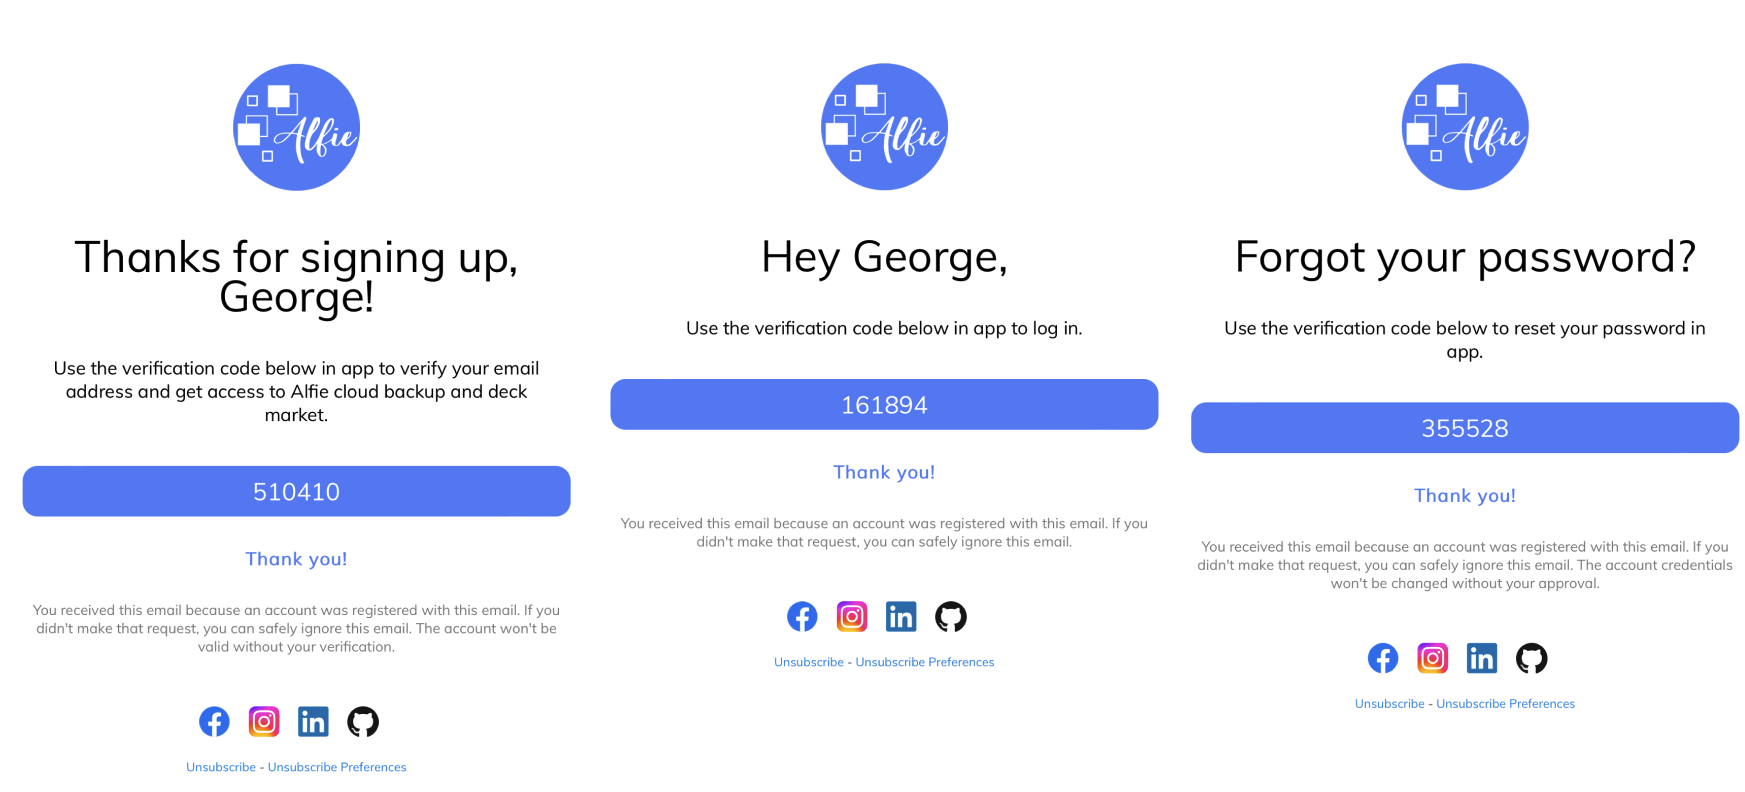
\includegraphics[width=\linewidth]{alfie-emails.png}
    \caption{Exemplu de email pentru verificarea unui cont de Alfie. Numele este înlocuit în template-ul dinamic de SendGrid cu cel al utilizatorului. Exemplu de email pentru verificarea logării unui cont. Exemplu de email pentru verificarea că cererea de resetare a parolei a fost realizată de titularul contului.}
    \label{fig:alfie_emails}
\end{figure}

Nu în ultimul rând, Twilio oferă mai multe SDK-uri pe lângă call-urile HTTP care permit folosirea lor în orice limbaj de programare suportat ori care pot realiza call-uri prin HTTP. Alfie folosește coduri de verificare cu o lungime de 6 cifre și o valabilitate de 10 minute. În cazul în care utilizatorul solicită un nou cod înainte de expirarea celor 10 minute, va fi trimis același email ce conține același cod \cite{twilioVerification}.

\subsubsection{Implementare în Go}

Alfie folosește SDK-ul de go pentru Twilio pentru a verifica email-uri \cite{twilioVerifyEmail}. În ceea ce privește păstrarea codului extensibil, modular și ușor de înlocuit, aplicația Alfie utilizează interfețe pentru toate serviciile sale. În cazul verificării email-urilor, Alfie definește o interfață a serviciului de \mintinline{go}{MailVerifierService} care necesită implementarea metodelor din codul sursă nr. \ref{code:go_mail_verifier_service} de mai jos.

În aplicația în Go se definește o structură care va integra metodele existente în interfața \mintinline{go}{MailVerifierService}. Totodată, este stabilită o funcție de creare a unui obiect ce implementează interfața și care conține informații despre cele trei id-uri ale serviciilor de verificare și din partea clientului de Twilio în go.

\begin{code}
    \inputminted[frame=single,framesep=2mm,linenos,breaklines,tabsize=2]{go}{code/mail-verifier-service.go}
    \captionof{listing}{Interfața pentru serviciul de verificarea a mail-urilor în Go}
    \label{code:go_mail_verifier_service}
\end{code}

\subsection{Salvarea conținutului media în cloud cu AWS S3}

Unul dintre feature-urile aplicației Alfie este acela de backup în cloud al cartonașelor și al conținutului media, fiind apelat în acest sens serviciul S3 oferit de AWS. AWS oferă SDK-uri pentru mai multe limbaje de programare, printre care și Go. În consola de AWS, Alfie dispune de un bucket special creat pentru acest proiect (numit \mintinline{tex}{alfie-gr}), ce este configurat astfel încât bucketul și obiectele din cadrul său să nu fie publice pentru a proteja datele utilizatorilor – block public access. De asemenea, acesta este configurat în regiunea Europa (Frankfurt). Bucketul folosește criptarea cheilor de tip SSE-S3.

Utilizatorii primesc acces folosind URL-uri presigned de către api. Astfel, api-ul în Go se asigură că fiecare utilizator dispune de accesul la informațiile care îi aparțin, fără a interfera cu cele ale altor utilizatori.

În S3 obiectele sunt salvate drept o cheie-valoare, unde cheia reprezintă un nume prefixat (în mod opțional) ca și o structură de directoare, iar valoarea este fișierul în sine.

\textbf{Structura bucket aws.} În S3 nu există foldere propriu-zise precum în alte sisteme de fișiere. În schimb, pentru organizare S3 suportă conceptul de foldere prin gruparea obiectelor în funcție de un prefix share-uit \cite{s3Folders}. Așadar, în cazul cheilor \mintinline{shell}{test/test1.txt} și \mintinline{shell}{test/test2.txt}, S3 va conține trei obiecte la cererea listării obiectelor din folderul \mintinline{shell}{test/} (folosind prefixul cheie):

\begin{enumerate}
    \item obiectul \mintinline{shell}{test/} care este gol și reprezintă "folderul"
    \item obiectul cu cheia \mintinline{shell}{test/test1.txt} care va fi considerat aparținând folderului \mintinline{shell}{test/}
    \item obiectul cu cheia \mintinline{shell}{test/test2.txt} care va fi considerat aparținând folderului \mintinline{shell}{test/}
\end{enumerate}

În felul acesta, Alfie definește două mari foldere în bucket, având scop organizatoric:
\begin{enumerate}
    \item \mintinline{shell}{backup/} – va conține o listă cu fișiere de backup ale bazelor de date aferente utilizatorilor;
    \item \mintinline{shell}{media/} – va conține o listă cu foldere dedicată fiecărui utilizator în parte. La crearea unui cont, utilizatorul primește un id unic de identificare pentru S3, pe lângă cel de cheie primară, id-ul utilizatorului putând fi folosit și în alte părți. În interiorul folderului se vor afla fișierele media ale utilizatorului.
\end{enumerate}

Api-ul de Alfie va genera un URL presemnat, prin intermediul căruia acesta (în calitate de autoritate asupra bucket-ului) dă permisiunea utilizatorului să încarce fișierul pentru care a efectuat o cerere. Api-ul autorizează URL-ul cu o valabilitate de timp care poate fi customizată, folosind variabila de environment \mintinline{shell}{PUT_FILE_EXPIRATION_TIME} pentru extensibilitate, întrucât această valoare trebuie să fie ajustată fără recompilarea programului. Dacă URL-ul expiră, atunci utilizatorul nu va mai putea încărca fișierul și va trebui să facă o nouă cerere \cite{s3PresignedUploadURL}.

Din moment ce a fost stabilit că bucketul este privat, api-ul de Alfie apelează din nou la URL-uri presemnate care îi conferă utilizatorului dreptul să descarce fișierul menționat în URL, atâta timp cât acesta este valid. La fel ca la încărcare, poate fi setată și o valabilitate în timp a URL-ului, cu ajutorul variabilei env \mintinline{shell}{DOWNLOAD_FILE_EXPIRATION_TIME}.

Api-ul cere utilizatorilor să fie autentificați în aplicația Alfie pentru a putea utiliza serviciul de media în cloud. Obținând token-ul de verificare al unui utilizator, api-ul îl caută în baza de date după adresa de email din claim-urile token-ului pentru a afla id-ul de S3 unic și a genera fișierul de backup cu cartonașele aferente acestui id. În felul acesta este imposibil ca un utilizator să primească backup-ul altor utilizatori. O situație similară apare și în cazul conținutului media, dat fiind faptul că este folosit id-ul de S3 unic al utilizatorului drept nume de folder. Așadar, în momentul încărcării de conținut media, un utilizator va putea încărca fișiere doar în folderul asignat acestuia. De asemenea, la descărcarea conținutului media, dacă utilizatorul cere fișiere care îi lipsesc local din cloud, api-ul verifică ca aceste fișiere să existe în folderul atribuit acestuia, și îi trimite link-uri doar pentru fișierele care îi aparțin și care există în cloud.

În mod similar cu implementarea pentru Twilio, Alfie definește o interfață a serviciului de cloud media pentru extensibilitate și posibilitatea de upgrade în viitor a unor noi versiuni și, respectiv, păstrarea usecase-ului. De asemenea, în interfață sunt definite funcții pentru usecase-urile prezentate (creare de fișier, listare de obiecte din fișier, generare link upload/download pentru un singur fișier/mai multe fișiere).

\begin{code}
    \inputminted[frame=single,framesep=2mm,linenos,breaklines,tabsize=2]{go}{code/media-cloud-service.go}
    \captionof{listing}{Interfața pentru serviciul de media cloud în Go}
    \label{code:go_media_cloud_service}
\end{code}

\section{3rd party OCR - serviciu în Node.js și TypeScript}

\subsection{OCR Mathpix}

Pentru transformarea imaginilor în text științific se apelează la un 3rd party api: serviciul \textbf{Mathpix OCR API}, întrucât OCR-ul este capabil să recunoască ecuații matematice, formule chimice, tabele și multe altele \cite{mathpixOCR}.

În cazul aplicației Alfie este nevoie de un sistem robust, testat în producție la scară mare. OCR-ul oferit de Mathpix dispune de mici latențe, având servere în trei regiuni principale ale lumii (America de Nord/America de Sud, Europa și Asia). Totodată, acesta poate procesa mai mult de 10 milioane de poze pe zi. Serviciile oferite de Mathpix sunt folosite și de alte nume importante în domeniu, precum Symolab și Facebook Research \cite{mathpixOCR}. Astfel, se dovedește a fi un serviciu potrivit pentru usecase-ul dorit de aplicația Alfie, motiv pentru care s-a obținut un api key pentru folosirea serviciului. Proiectul Alfie va utiliza acest OCR pentru convertirea imaginilor în text de tip TeX cu scopul creării cartonașelor.

Pentru apelarea api-ului sunt necesare următoarele secrete: id-ul aplicației ce este generat în dashboardul mathpix și api key-ul \cite{mathpixApiReqParam}. În continuare, server-ul de express este configurat de așa manieră încât să se comporte ca un proxy între client (aplicația de mobil) și serviciul 3rd api, dat fiind faptul că aceste secrete nu trebuie să fie făcute publice.

Astfel, se definește o rută pe care pot fi primite fișiere folosind request-uri de tip multipart din partea clienților. Această rută este interceptată pe server-ul de express de un middleware de autentificare care forțează caller-ul să fie autentificat prin oferirea tokenului de auth. În lipsa acestuia, middleware-ul întoarce răspunsul negativ la client. Dacă utilizatorul este autentificat în aplicație, middleware-ul trimite apelul către controller.

La rândul său, controller-ul citește buffer-ul pentru fișier și trimite imaginea către o clasă serviciu pentru apelul 3rd api. În cadrul serviciului, imaginea va fi comprimată până la un target de maxim 100Kb. Compresia este de tip JPEG și se realizează folosind librăria \mintinline{tex}{sharp} \cite{sharpImageCompression}. Motivul ce stă la baza alegerii acestei librării în detrimentul altor variante la fel de populare, cum ar fi ImageMagick sau GraphicsMagik, constă în faptul că este mai rapidă, în comparație cu acestea (chiar și de 4-5 ori mai rapidă) \cite{sharpImageCompression}. În felul acesta, serviciul se folosește de compresia JPEG pentru a genera imaginea comprimată într-un buffer. Acest lucru se realizează într-un loop în funcție de factorul de comprimare a calității (care pornește de la 95 și se duce până la minim 5) pentru a verifica mărimea imaginii comprimate rezultate până când se obține target-ul dorit, și anume cel de maxim 100Kb. Fiecare pas implică o scădere cu 5 procente a factorului calității.

În final, este apelat api-ul Mathpix cu un request multipart pentru a trimite imaginea comprimată, iar la acest apel se adaugă și alte informații pentru customizarea rezultatului. Este setat un treshold pentru confidența că api-ul a compus corect textul din imagine, fiind stabilit la 85\%. Astfel, serviciul este configurat să întoarcă înapoi eroarea, în cazul în care output-ul nu este cel dorit, iar clientul să realizeze o fotografie cu o claritate mai ridicată. De asemenea, textul în TeX dispune de câteva opțiuni specificate pentru formatarea acestuia, și anume: să fie între simbolurile ’\$\$’ pentru a centra rezultatul în centrul cartonașului, precum și pentru a șterge spațiile în plus realizate de api între caractere. Răspunsul este întors de serviciu către controller și, ulterior, către client.

În cazul în care apar diverse erori datorită compresiei sau a 3rd party api-ul, acestea sunt prinse și logate, iar aplicația termină apelul fără a provoca alte incidente.

Pentru a evita traficul excesiv, serverul de express folosește un rate limiter. Motivul pentru care este implementat un rate limiter în cazul acestui serviciu este acela de a preveni traficul rău intenționat care ar încerca să abuzeze de resursele sistemului, dat fiind faptul că serviciul utilizează mult trafic de internet pentru trimiterea pozelor, dar și resurse pentru comprimarea lor în cazul multor cereri. Cu ajutorul acestei soluții este limitat numărul de resurse folosit în mod abuziv, fără a diminua experiența utilizatorului, din moment ce acestuia îi va lua destul de mult timp să creeze un cartonaș și intervalul rate limiterului este unul rezonabil de sub 15 secunde. Acest rate limiter se bazează pe adresa ip a apelantului. Prin intermediul variabilelor de enviroment ale aplicației poate fi definit și numărul de request-uri într-o anumită perioadă de timp. Dacă un client realizează mai multe apeluri în acest interval, serverul va ignora celelalte cereri și nu va realiza nicio procesare dificilă (costisitoare).

\subsection{Node.js \& TypeScript}

În ceea ce privește feature-ul de obținere a ecuațiilor matematice din poze în TeX, proiectul Alfie apelează la un serviciu care se va ocupa doar de acest lucru. Unul dintre argumentele ce ar trebui menționate este reprezentat de faptul că aplicația separată va fi scalată diferit de cea principală, întrucât acest serviciu se va ocupa doar de primirea și trimiterea pozelor sau, cu alte cuvinte, de heavy networking, respectiv de compresia imaginilor. Totodată, se dorește ca dezvoltarea lui să fie rapidă și simplă, motiv pentru care este ales un server în Node.js cu framework-ul express pentru realizarea acestuia.

Nu în ultimul rând, pentru dezvoltarea acestui server este utilizat limbajul TypeScript în loc de JavaScript, având în vedere că, fiind un limbaj static typed, acesta este mult mai avantajos în ceea ce privește dezvoltarea serverului respectiv, oferind mai multe informații, precum obținerea mai eficientă a tipurilor de date și erori. La final se va converti codul din TypeScript în cod de JavaScript pentru a fi rulat de serverul Node.js, acesta fiind mai eficient decât serverul Node de TypeScript.

\section{Docker și deploy producție}

\subsection{Docker}

Docker reprezintă o platformă open source dedicată pentru dezvoltarea, livrarea și rularea aplicațiilor, care oferă capacitatea de a crea și a rula aplicații în medii izolate, numite containere. Aceste containere sunt mici, conținând toate dependențele de care are nevoie o aplicație ca să ruleze \cite{docker}.

Dat fiind faptul că aplicațiile pot fi containerizate alături de toate dependențele necesare într-un mediu izolat, acestea sunt partajate de pe un calculator pe celălalt, garantând păstrarea identică a modului de funcționare specific containerului respectiv. Din acest motiv, containerele sunt considerate ca fiind foarte eficiente în procesul de dezvoltare, permițând crearea cu ușurință a unui nou setup între membrii echipei de lucru.

În containere poate avea loc atât rularea imaginilor puse la dispoziție pe DockerHub, cât și construirea propriilor imagini ale aplicațiilor.

Pentru proiectul Alfie se folosește un fișier \mintinline{shell}{Compose} prin care se vor defini serviciile sistemului, rețeaua de comunicație între servicii, volumele disponibile pentru fiecare serviciu în parte, precum și environment-ul. Alfie utilizează Docker atât pentru development, cât și pentru production, ambele acțiuni fiind justificate prin faptul că permite crearea unui environment stabil și identic în cazul tuturor dezvoltatorilor (cu toate că acesta a fost creat doar de către autorul prezentei lucrări, care crede în gândirea extensibilă).

Fișierul de Compose pentru development este redat în codul sursă nr. \ref{code:docker_compose} de mai jos:

\begin{code}
    \inputminted[frame=single,framesep=2mm,linenos,breaklines,tabsize=2]{yaml}{code/compose.yaml}
    \captionof{listing}{Fișier Docker Compose pentru proiectul Alfie}
    \label{code:docker_compose}
\end{code}

Acest fișier este extins spre partea de production cu ajutorul fișierului de tip Compose: \mintinline{shell}{compose.prod.yaml} din codul sursă nr. \ref{code:docker_compose_prod}, având setările specifice producției. Printre aceste setări se numără încărcarea certificatului și a cheii private pentru a fi folosite de servicii, dar și configurararea bazei de date, astfel încât să accepte doar conexiuni prin TLS către outside world.

\begin{code}
    \inputminted[frame=single,framesep=2mm,linenos,breaklines,tabsize=2]{yaml}{code/compose.prod.yaml}
    \captionof{listing}{Fișier adițional Docker Compose Prod pentru proiectul Alfie}
    \label{code:docker_compose_prod}
\end{code}

Pentru networking-ul între servicii este definită o rețea privată prin intermediul fișierului de compose: \mintinline{yaml}{alfie_network} de subnet \mintinline{yaml}{172.21.10.0/24}. Rețeaua este delimitată cu ajutorul unei măști pe 24 de biți în locul uneia de 16 biți, ce apare configurată în mod predefinit de Docker, astfel încât să fie puse la dispoziție cât mai multe astfel de subrețele. În momentul de față, proiectul Alfie folosește doar trei servicii, iar fiecare serviciu este conectat la această rețea, fiindu-i alocată o adresă IPv4. Astfel faptul că rețeaua este limitată la 256 de adrese IP nu reprezintă o problemă.

Fișierul de Compose conține următoarele trei servicii:
\begin{enumerate}
    \item \textbf{O bază de date PostgreSQL.} Această bază de date este configurată cu variabile de environment pentru a masca secretele din codul sursă care va fi expus. Containerul este conectat la rețeaua \mintinline{yaml}{alfie_network}, fiindu-i alocată adresa \mintinline{yaml}{172.21.10.2}. Baza de date rulează în container și folosește portul \mintinline{yaml}{5432} intern, iar containerul expune către host portul \mintinline{yaml}{21092} pentru a accesa baza de date.

    \item \textbf{Backendul in Go.} Containerul folosește o imagine care va fi construită conform fișierului Dockerfile din folderul \mintinline{yaml}{./api}. Serviciul este conectat la rețeaua \mintinline{yaml}{alfie_network}, fiindu-i alocată adresa \mintinline{yaml}{172.21.10.3} și depinde de cel al bazei de date. Aplicația rulează în container și folosește portul \mintinline{yaml}{8080} intern, iar containerul expune către host portul \mintinline{yaml}{21093} pentru acces.

    Fișierul de build pentru aplicația în Go se va folosi de ultima imagine de pe \textit{DockerHub} de Golang. În primul rând, config-ul va descărca dependențele aplicației cu ajutorul sistemului de versioning oferit de Go. Ulterior, config-ul va obține dependențele necesare pentru compilatorul de protobuf și va genera fișierele de Go din serviciul \mintinline{protobuf}{Alfie} configurat în protobuf. După ce toate dependențele sunt rezolvate, config-ul va compila aplicația și va rula executabilul creat.
    
    \item \textbf{Serviciul de OCR pentru TeX în Node.js.} Containerul utilizează o imagine ce va fi construită conform fișierului Dockerfile din folderul \mintinline{yaml}{./math_ocr_api}. Serviciul este conectat la rețeaua \mintinline{yaml}{alfie_network}, fiindu-i alocată adresa \mintinline{yaml}{172.21.10.4} și depinde de ambele servicii menționate mai sus. Aplicația rulează în container și folosește portul \mintinline{yaml}{8085} intern, iar containerul expune către host portul \mintinline{yaml}{21094} pentru access.
    
    Fișierul de build pentru aplicația în Node.js se va folosi de imaginea \textit{node:16-alpine} de pe \textit{DockerHub}. În primul rând, config-ul va descărca dependențele aplicației cu ajutorul sistemului de versioning oferit de \mintinline{shell}{yarn}. Ulterior, config-ul va rula un script de yarn pentru a realiza build-ul de producție ce va converti aplicația din cod de TypeScript în cod de JavaScript.
    
    La final, aplicația va rula script-ul yarn de rulare a aplicației în producție.
\end{enumerate}

\subsection{Securitatea comunicațiilor dintre client și server}

Un alt factor important al securității este reprezentat de \textit{comunicarea criptată}. Configurațiile descrise până în acest punct nu au nicio proprietate care să permită realizarea criptării mesajelor atunci când sunt comunicate. Acest lucru vine în favoarea unui atacator pasiv care doar urmărește comunicațiile dintre un client și un server pentru a afla mesajele schimbate între ei. Pe lângă încălcarea privacy-ului clientului, există și o breșă de securitate. Atacatorul ar avea posibilitatea de a vedea mesajul de logare al utilizatorului, identificând atât credențialele pentru email și parolă, cât și token-ul de autentificare, ceea ce îi permite să impersoneze clientul.

Pe fondul acestor justificări, s-a luat decizia de a implementa măsuri de securitate și de configurare a sistemului proiectului Alfie în așa manieră încât să poată comunica și criptat. Trebuie menționat faptul că nu este nevoie de o comunicație criptată în mediul de dezvoltare, din moment ce sistemul nu este publicat, astfel că dezvoltatorul trebuie să se asigure pe cont propriu că sistemul său nu este compromis.

Sistemul configurat în producție comunică cu exteriorul prin TLS. În acest scop a fost achiziționat un certificat de la un furnizor autorizat de certificate. Astfel, clienții Alfie vor avea certitudinea că aplicația de mobil comunică cu serviciile corecte de cloud, dar și faptul că aceste  comunicații realizate cu serverul sunt criptate.

În felul acesta, se ajunge la două nevoi separate de environment și un singur cod sursă. Pentru a folosi același cod atât în producția cu comunicații securizate, cât și în dezvoltarea cu comunicații nesecurizate, se apelează la o variabilă de environment ce menționează aplicațiilor atunci când să ruleze în modul de producție, iar în funcție de acest lucru vor fi create canale de comunicație diferite pentru fiecare caz.

În ceea ce privește realizarea comunicațiilor securizate în Go, se încarcă credențialele \mintinline{shell}{x509} din fișierul certificat și cheia privată și sunt atașate serverului de gRPC.

\begin{code}
    \inputminted[frame=single,framesep=2mm,linenos,breaklines,tabsize=2]{go}{code/tls-grpc-go.go}
    \captionof{listing}{Configurarea unui canal de comunicații securizat folosind TLS și gRPC în Go}
    \label{code:go_grpc_tls}
\end{code}

Pentru a realiza comunicații securizate în Node.js, se încarcă certificatul și cheia privată și se folosește modulul \mintinline{js}{https} în loc de \mintinline{js}{http}.

\begin{code}
    \inputminted[frame=single,framesep=2mm,linenos,breaklines,tabsize=2]{javascript}{code/tls-https-node-js.js}
    \captionof{listing}{Configurarea unui canal de comunicații securizat folosind TLS și express în Node.js}
    \label{code:node_https_tls}
\end{code}

De asemenea, clientul de Flutter este instruit să comunice doar prin canale securizate.

\begin{code}
    \inputminted[frame=single,framesep=2mm,linenos,breaklines,tabsize=2]{dart}{code/tls-client.dart}
    \captionof{listing}{Clientul este instruit să accepte doar canale securizate când comunică prin gRPC}
    \label{code:client_tls}
\end{code}

Este important de menționat faptul că baza de date nu ar trebuie să fie accesibilă în exterior, dat fiind faptul că este deja disponibilă în docker prin rețeaua definită. Totuși, se dorește vizualizarea datelor pentru development, respectiv pentru verificarea datelor și a funcționalităților, motiv pentru care a fost expus și portul bazei de date către exterior din docker. În felul acesta, a fost publicată și baza de date, accesul fiind efectuat prin autentificare pe bază de user și parolă, fără criptarea implicită, ceea ce produce vulnerabilități și un risc major. Având în vedere acest lucru, a fost creat și un config pentru inițializarea bazei de date, astfel încât să poată fi folosit TLS. De asemenea, în config, baza de date este configurată să comunice cu exteriorul doar prin TLS, nefiind permis într-un alt mod. În cazul serverului unde este rulat containerul sunt acceptate ambele metode, dat fiind faptul că persoanele care au acces la instanță au acces la tot. Dacă cineva neautorizat obține accesul la instanță, acest lucru poate cauza oricum probleme mai grave.

Securizarea instanței reprezintă un alt subiect de discuție. Comunicațiile se fac prin protocolul de rețea \mintinline{shell}{SSH}. Accesul la cheia privată pentru conectarea prin SSH să fie acordat unui număr mic de persoane autorizate.

\subsection{Deployment live și CI/CD}

Odată dezvoltat proiectul, acesta trebuie să ajungă și în producție, iar până în acest moment au fost realizate configurații pentru a îndeplini acest scop.

Containerele de docker sunt deployate pe o instanță de EC2 oferită de serviciile de la AWS. Instanța de EC2 rulează Amazon Linux 2 ca sistem de operare, fiindu-i alocat un IP elastic din consola de la AWS. Pentru conectarea la instanța de linux din cloud, dezvoltatorul se folosește de protocolul \mintinline{shell}{SSH}. Acesta este securizat, accesul realizându-se doar cu ajutorul unei chei private generată folosind \mintinline{shell}{openssh} în consola de AWS. Instanța de linux are unelte de bază (printre care editorul de text Vi în terminal), motiv pentru care autorul lucrării de față a instalat aplicațiile necesare pentru funcționare, cum ar fi \mintinline{shell}{git}, \mintinline{shell}{docker}.

De asemenea, pe această instanță a fost generat un request pentru certificat (CSR) cu informațiile despre proiect și organizație. Ulterior, acest request a fost transmis în interfața unei autorități de certificate pentru generarea certificatului. După descărcarea certificatului, acesta a fost instalat pe server pentru comunicații securizate prin TLS. Aceste fișiere sunt configurate cu permisiuni de read și write only (cod permisiuni 640).

Pentru automatizarea procesului de publicare a noilor actualizări ale serviciilor de cloud este configurat un pipeline. Pipeline-ul este definit cu ajutorul GitHub Actions care se va declanșa pentru actualizările de pe branchul \mintinline{shell}{main}, fiind configurat încât să obțină variabile de environment din GitHub Secrets, stabilite la nivel de repository. Secretele reprezintă informațiile de acces pentru instanța de EC2 unde este configurat sistemul. După realizarea conexiunii de SSH, pipeline-ul va actualiza versiunea proiectului Alfie de pe instanța de EC2 folosind CLI-ul de git și va actualiza imaginile de docker. De asemenea, acesta va curăța versiunile vechi ale imaginilor pentru a optimiza spațiul de stocare deja ocupat.

\chapter{Concluzii}

\textbf{Dezvoltări ulterioare.} Printre alte feature-uri ce ar îmbunătăți aplicația Alfie se numără extinderea conținutului media permis pentru fiecare cartonaș în parte, prin adăugarea unui suport pentru audio, integrarea cu un serviciu de traducere, dar și cu un serviciu de partajare a pachetelor de cartonașe. Alte dezvoltări ar putea include și lansarea proiectului pe telefoanele mobile cu sistem de operare iOS din build-ul curent de Flutter, respectiv realizarea de build-uri pentru sisteme de operare de desktop.

\textbf{Experiența utilizatorului} Aplicația \textit{Alfie} a fost gândită și testată intensiv prin prisma unui utilizator normal, motiv pentru care interfața este una simplă și intuitivă. Autorul prezentei lucrări intenționează să adauge mai multe feature-uri și customizări aplicației, ținând cont de experiența utilizatorului final. Prin aplicația Alfie s-a reușit oferirea unui suport mai bun pentru cartonașe în rândul elevilor și al studenților din domeniul științific, implementarea serviciului de OCR fiind complet funcțională. De asemenea, cartonașele oferă extensibilitatea dorită prin cele patru tipuri de format pentru text și conținutul media integrat, iar sistemul de backup este unul funcțional și eficient. Nu în ultimul rând, sistemul creat suportă o varietate de tehnologii și integrări, cum ar fi cea de email pentru 2FA și backup media.

\textbf{Experiența autorului} Prin crearea și dezvoltarea acestui proiect, am încercat să acopăr cât mai multe aspecte și principii specifice dezvoltării software și de realizare a unui produs, astfel că au ajuns să fie incluse mai multe tehnologii distincte ca principii pentru a-mi demonstra capacitatea ridicată de adaptare. Totodată, am urmat principiile de bază în dezvoltarea de software, am adăugat multe feature-uri, dar am păstrat un cod clean, ușor de înțeles și extensibil.

În felul acesta, am reușit să acopăr mai multe domenii abordate în cadrul studiilor mele universitare, pornind de la algoritmi, structuri de date, baze de date, inginerie software, networking și securitate, demonstrând prin aplicația \textit{Alfie} capacitatea proprie și profesională.


\begin{appendix}
\chapter{Folosirea GORM în cadrul api-ului în Go}

\label{annex:gorm}

\begin{code}
    \inputminted[frame=single,framesep=2mm,linenos,breaklines,tabsize=2]{go}{code/go-gorm.go}
    \captionof{listing}{Conectarea la baza de date folosind GORM și rularea migrațiilor}
    \label{code:go_connect_database_and_migrations}
\end{code}

\begin{code}
    \inputminted[frame=single,framesep=2mm,linenos,breaklines,tabsize=2]{go}{code/go-user-model.go}
    \captionof{listing}{Definirea modelului de user folosind GORM din api-ul de GO}
    \label{code:go_user_model_gorm}
\end{code}


\end{appendix}

\printbibliography[heading=bibintoc]

\end{document}